\documentclass[anon,12pt]{colt2021} % Anonymized submission
%\documentclass[final]{colt2020} % Anonymized submission
% \renewcommand{\includegraphics}[1][1]{}

% \documentclass{colt2020} % Include author names

% The following packages will be automatically loaded:
% amsmath, amssymb, natbib, graphicx, url, algorithm2e


\usepackage{times}

\usepackage{lmodern}
\usepackage{hyperref}       % hyperlinks  %[implicit=false, bookmarks=false]
\usepackage{booktabs}       % professional-quality tables
\usepackage{amsfonts}       % blackboard math symbols
\usepackage{nicefrac}       % compact symbols for 1/2, etc.
\usepackage{microtype}      % microtypography

\PassOptionsToPackage{numbers, sort, compress}{natbib}

\usepackage{mathtools, verbatim}
%\usepackage[thmmarks, thref, amsthm]{ntheorem}
\usepackage{color}
\definecolor{darkblue}{rgb}{0.0,0.0,0.2}
\hypersetup{colorlinks,breaklinks,
	linkcolor=darkblue,urlcolor=darkblue,
	anchorcolor=darkblue,citecolor=darkblue}
\usepackage{wrapfig}
\usepackage{caption}
% NOTE: had to comment out "todo" in colt2021.cls
\usepackage[colorinlistoftodos,textsize=tiny]{todonotes} % need xargs for below
%\usepackage{accents}
\usepackage{bbm}
\usepackage{xspace}

\makeatletter
\let\Ginclude@graphics\@org@Ginclude@graphics 
\makeatother

%\usetikzlibrary{calc}
\newcommand{\Comments}{1}
\newcommand{\mynote}[2]{\ifnum\Comments=1\textcolor{#1}{#2}\fi}
\newcommand{\mytodo}[2]{\ifnum\Comments=1%
	\todo[linecolor=#1!80!black,backgroundcolor=#1,bordercolor=#1!80!black]{#2}\fi}
\newcommand{\raf}[1]{\mynote{green}{[RF: #1]}}
\newcommand{\raft}[1]{\mytodo{green!20!white}{RF: #1}}
\newcommand{\jessie}[1]{\mynote{purple}{[JF: #1]}}
\newcommand{\jessiet}[1]{\mytodo{purple!20!white}{JF: #1}}
\newcommand{\bo}[1]{\mynote{blue}{[Bo: #1]}}
\newcommand{\botodo}[1]{\mytodo{blue!20!white}{[Bo: #1]}}
\newcommand{\btw}[1]{\mytodo{orange!80!white}{BTW: #1}}
\newcommand{\discuss}[1]{\mynote{cyan!20!white}{#1}}
\ifnum\Comments=1               % fix margins for todonotes
\setlength{\marginparwidth}{1in}
\fi

\newcommand{\reals}{\mathbb{R}}
\newcommand{\posreals}{\reals_{>0}}%{\reals_{++}}
\newcommand{\simplex}{\Delta_\Y}
\newcommand{\relint}[1]{\mathrm{relint}(#1)}
\newcommand{\interior}{\mathrm{int}\,}
\newcommand{\prop}[2][\mathcal{P}]{\mathrm{prop}_{#1}[#2]}
\newcommand{\elic}{\mathrm{elic}}
\newcommand{\eliccvx}{\mathrm{elic}_\mathrm{cvx}}
\newcommand{\elicpoly}{\mathrm{elic}_\mathrm{pcvx}}
\newcommand{\elicembed}{\mathrm{elic}_\mathrm{embed}}
\newcommand{\ccdim}{\mathrm{cc\,dim}}
\newcommand{\rank}{\mathrm{rank}}
\newcommand{\proj}{\mathrm{proj}}
\newcommand{\supp}{\mathrm{supp}}
\newcommand{\spn}{\mathrm{span}}

\newcommand{\range}{\mathrm{range}\,}
\newcommand{\zeros}[1]{\mathrm{ker}_\P\,#1}
\newcommand{\codim}{\mathrm{codim}}
\newcommand{\Pcodim}{\mathcal{P}\!\text{-}\mathrm{codim}}
\newcommand{\Pcodimension}{$\mathcal{P}$-codimension\,}

\newcommand{\propdis}{\mu}
\newcommand{\affhull}{\mathrm{affhull}}
\newcommand{\epi}{\mathrm{epi}}
\newcommand{\cl}{\mathbf{cl}}
%\newcommand{\span}{\mathrm{span}}

\newcommand{\A}{\mathcal{A}}
\newcommand{\C}{\mathcal{C}}
\newcommand{\D}{\mathcal{D}}
\newcommand{\E}{\mathbb{E}}
\newcommand{\F}{\mathcal{F}}
\renewcommand{\L}{\mathcal{L}}
\newcommand{\I}{\mathcal{I}}
\newcommand{\N}{\mathcal{N}}
\newcommand{\R}{\mathcal{R}}
\renewcommand{\P}{\mathcal{P}}
\newcommand{\Sc}{\mathcal{S}}  % jessie, feel free to redef, just not \S :-)
\newcommand{\Scr}{\mathcal{S}}  % using this for the span of F_p - not sure if we want this to be parallel to the feasible subspace notation
\newcommand{\U}{\mathcal{U}}
\newcommand{\X}{\mathcal{X}}
\newcommand{\Y}{\mathcal{Y}}


\newcommand{\ellbar}{\underline{\ell}}
\newcommand{\lbar}{\underline{L}} % couldn't do L* while proofreading...
\newcommand{\iden}{\mathrm{iden}}
\newcommand{\im}{\mathrm{im}}
\newcommand{\Var}{\mathrm{Var}}
\newcommand{\CVaR}{\mathrm{CVaR}}

\newcommand{\exploss}[3]{\E_{#3} #1(#2,Y)}
\newcommand{\risk}[1]{\underline{#1}}
\newcommand{\Ind}[1]{\mathbf{I}\{{#1}\}}
\newcommand{\inprod}[2]{\langle #1, #2 \rangle}
\newcommand{\toto}{\rightrightarrows}
\newcommand{\ones}{\mathbbm{1}}

%\newtheorem{theorem}{Theorem}
%\newtheorem{lemma}{Lemma}
%\newtheorem{proposition}{Proposition}
%\newtheorem{corollary}{Corollary}
%\newtheorem{conjecture}{Conjecture}
%\newtheorem{definition}{Definition}
\newtheorem{assumption}{Assumption}
\newtheorem{condition}{Condition}
%\newtheorem{remark}{Remark}


\DeclareMathOperator*{\argmax}{arg\,max}
\DeclareMathOperator*{\argmin}{arg\,min}
\DeclareMathOperator*{\arginf}{arg\,inf}
\DeclareMathOperator*{\sgn}{sgn}

\usepackage{thmtools, thm-restate}
%\declaretheorem{corollary}



% The \author macro works with any number of authors. There are two commands
% used to separate the names and addresses of multiple authors: \And and \AND.
%
% Using \And between authors leaves it to LaTeX to determine where to break the
% lines. Using \AND forces a line break at that point. So, if LaTeX puts 3 of 4
% authors names on the first line, and the last on the second line, try using
% \AND instead of \And before the third author name.

%Indirect elicitation as a necessary condition for consistent surrogate losses
\title{Unifying Lower Bounds on Prediction Dimension of Consistent Convex Surrogates}

% Three or more authors with the same address:
\coltauthor{\Name{Jessie Finocchiaro} \Email{jessica.finocchiaro@colorado.edu}\\
	\Name{Rafael Frongillo} \Email{raf@colorado.edu}\\
	\Name{Bo Waggoner} \Email{bwag@colorado.edu}\\
	\addr CU Boulder}


\begin{document}

\maketitle

\begin{abstract}
Given a prediction task, understanding when one can and cannot design a consistent convex surrogate loss, particularly a low-dimensional one, is an important and active area of machine learning research. 
Surrogate loss construction often presents itself in one of two scenarios, typically studied by different frameworks: first, when one is given a target loss for a finite prediction task, and second, when one simply has a statistic they would like to estimate.
%Through indirect property elicitation, we present a tool to study bounds on prediction dimension for surrogates in both of these settings.
Motivated by settings such as structured prediction where the prediction dimension of the surrogate is of central\jessiet{a tad dramatic?} importance, we give a new technique for constructing lower bounds on the convex prediction dimension that applies to both frameworks. 
Our lower bound tightens existing results in the case of discrete predictions, namely the feasible subspace dimension of~\citet{ramaswamy2016convex}, showing that previous calibration-based bounds can largely be recovered via property elicitation.
For statistic estimation, our lower bound gives new results for estimating variance as well as the entropy and norms of the conditional distribution.
%
%
%Given a prediction task, understanding when one can and cannot design a consistent convex surrogate loss, particularly a low-dimensional one, is an important and active area of machine learning research. 
%While calibration has historically been used to reason about consistency, we propose indirect property elicitation as an alternative necessary condition for a surrogate loss to be consistent. 
%Motivated by structured prediction and other domains where the prediction dimension of the surrogate is of central importance, we give a novel lower bound on the prediction dimension. 
%Our lower bound tightens existing results in the case of discrete predictions, namely the feasible subspace dimension, showing that previous calibration-based bounds can largely be recovered purely via property elicitation.
%For continuous predictions, our lower bound gives new results for variance estimation as well as the estimation of entropy and norms of the conditional distribution.
\end{abstract}

\section{Introduction}\label{sec:intro}
%supervised learning blah
Surrogate risk minimization is one of the most widespread learning heuristics in supervised machine learning.
%A surrogate loss is often necessary for one of two reasons: (1) the target loss does not satisfy some desiderata, such as convexity, or (2) the target loss may not be given at all, as is often the case in continuous estimation problems, when one instead has a target conditional statistic to estimate from training data.
Often, we desire surrogate losses to be \emph{consistent}, which informally means the surrogate loss ``corresponds'' to the desired learning problem, and this condition is a prerequisite for deriving excess risk bounds.
%Deriving excess risk bounds and rates require a surrogate to be consistent, hence the focus on consistency.
Construction of surrogates for a desired task is often ad hoc, leaving consistency of such losses an open question.
Depending on the data distribution, these inconsistent surrogates may actually yield high misprediction rates. \jessiet{Clean this up.}
%Roughly speaking, consistency means that minimizing surrogate risk corresponds to solving the target problem of interest: the target risk should also be minimized, or the average deviation from the true conditional statistic function converges to 0.\jessie{Not sure if I like these sentences here, or in general}

%examples of problems where we care a lot about prediction dimension (that happen to be finite discrete)
A variety of prediction tasks call for the construction of consistent, and ideally convex, surrogates.
Applications ranging from extreme classification to top-$k$ predictions to ranking have inspired an entire line of research into the construction of surrogate loss functions for such discrete tasks.
The dimensionality of such surrogate prediction space often scales linearly with the number of outcomes unless sacrifices are made in terms of consistency if one is not careful.
This linear growth of prediction dimension (in the number of outcomes) leads to computationally expensive or intractable optimization problems, but it is unknown in many cases if this linear scaling in dimensionality is necessary for a consistent surrogate.
Tight bounds on the dimension of the prediction space for a consistent convex surrogate remain an open question.

For some tasks, it is possible to reduce the dimension of this surrogate prediction space without sacrificing consistency.  
Consider the high-confidence classification presented by the abstain target loss~\citep{ramaswamy2012classification,ramaswamy2018consistent}.
When trying to predict one of $n$ outcomes, the abstain loss is minimized by predicting the most likely outcome if it is likely enough, and ``abstaining'' from predicting otherwise.
\citet{ramaswamy2016convex} present a convex surrogate, called the BEP loss, for the abstain target loss that takes as input a prediction whose dimension is logarithmic in the number of outcomes.
The BEP loss is a high-dimensional generalization of the hinge loss so that outcome predictions are ``embedded'' into the corners of the $\pm 1$ hypercube, and abstaining is embedded to the origin.
This BEP loss is consistent with respect to the target 0-1 modification $\ell(r,y) = \Ind{r \not \in \{y,\bot\}} + (1/2) \Ind{r = \bot}$, and takes $\Theta(\log n)$-dimensional surrogate predictions, instead of $\Theta(n)$, as was required of previous consistent surrogates.\jessie{Some of this repetitive}


%in a seemingly unrelated setting, finance problems blah blah.
In its own line of literature, financial institutions have sought scoring rules to learn banks' estimates of financial risk in their investments.\jessie{cite}
Given the desired measure of financial risk, such as the variance or Conditional Value at Risk (CVaR), auditing institutions are tasked with designing scoring rules that, directly or indirectly, incentivize truthfully estimating the desired statistic.
For example, while there is no loss function that enables one to directly learn the variance, we can learn the first and second central moments \jessiet{how much detail to share?} by proper scoring rules, which yields an unbiased estimator of the variance.
However, asking a bank for a large number of predictions may be infeasible by their own knowledge of the financial risk distribution.
That is, institutions and individuals might only be reasonably expected to articulate summary statistics of their beliefs, rather than their entire belief distribution.
To this end, learning desired statistics with a minimal number of reports also emerges as an important question in finance.
\jessie{Raf, helppp}


% point out distinctions and how these seem like very different settings (e.g. loss vs no loss), but we'll be able to address both with the same techniques, modulo some simplicity in the proofs.
The two examples above are seemingly unrelated given how different the settings are; in the abstain problem, we have a finite prediction problem where we want to design a consistent convex surrogate for a given target loss.
In risk estimation, on the other hand, we aim to estimate a continuous variable based on the desired summary statistic instead of target loss.
These two types of problems have been historically studied with different mathematical tools because of these perceived differences; however, in this paper, we show formal connections between consistent surrogates and property elicitation, and leverage these to understand new bounds on prediction dimension for consistent surrogates that spans both settings. 

\paragraph{The ``four quadrants'' of problem types}
Above, we discuss a significant divergence in previous frameworks: the difference in constructing a surrogate given a \emph{target loss} and a \emph{target statistic}.
In addition to the two possible targets, we may have one of two domains: a \emph{discrete} (i.e.\ finite) target prediction space, like a classification problem, or a \emph{continuous} one, like a regression or estimation problem.
We informally refer to the four resulting cases---target loss vs.\ target statistic, and discrete vs.\ continuous predictions---as the ``four quadrants'' of supervised learning problems, shown in Figure~\ref{fig:four-quadrants}.
For further examples in the off-diagonal quadrants, see Appendix~\ref{app:omitted-examples}.

\begin{figure}
	\begin{minipage}{0.25\linewidth}
	\caption{The four quadrants of prediction tasks; Theorem~\ref{thm:consistent-implies-indir-elic} allows us to understand the relationship between indirect elicitation and consistency in all four quadrants for the first time.}\label{fig:four-quadrants}	
	\end{minipage}
	\hfill
	\begin{minipage}{0.72\linewidth}
	\centering
	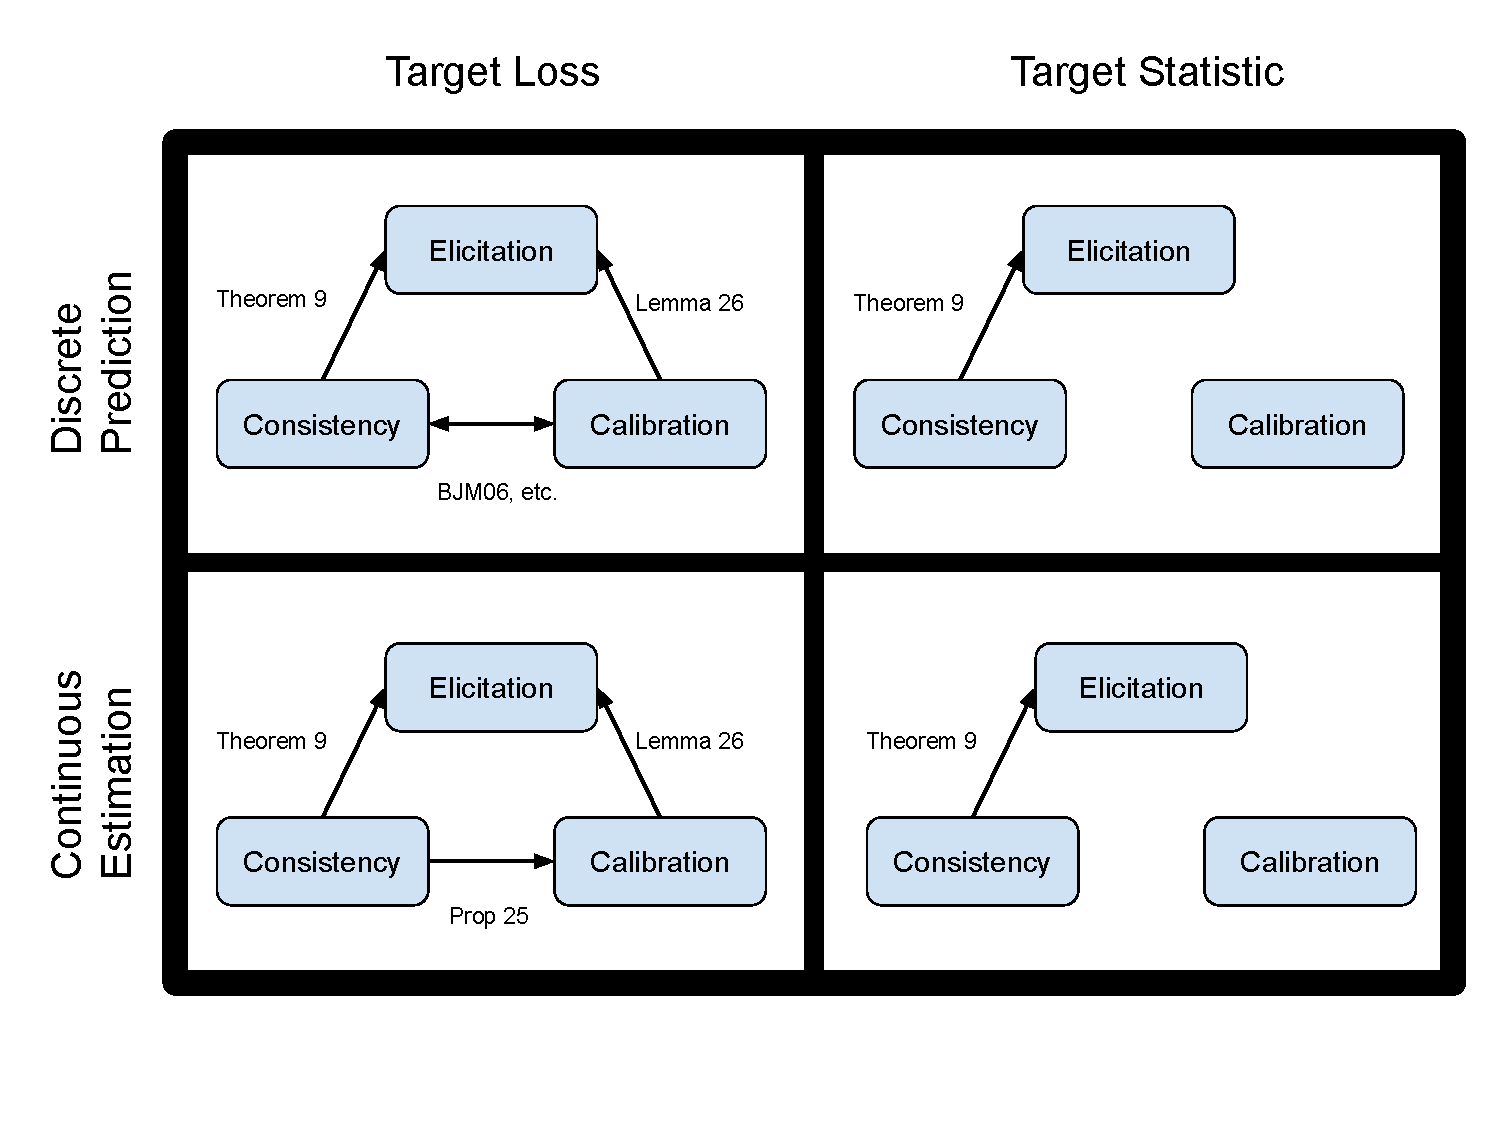
\includegraphics[width=0.95\linewidth]{tikz/consistency-elicitation-calibration.pdf}
	\end{minipage}
\end{figure}


\paragraph{Contributions}
\jessiet{Almost definitely want to re-format and polish this.}
Our contributions are as follows:
\begin{itemize}
	\item Formalize a notion of consistency with respect to a target statistic (Definition~\ref{def:consistent-prop}) and show its relationship to consistency with respect to a target loss (Lemma~\ref{lem:consistent-loss-implies-prop}).
	\item Show indirect elicitation is a necessary condition for consistency (Theorem~\ref{thm:consistent-implies-indir-elic}).
	\item Present a new framework for deriving lower bounds on the prediction dimension of consistent convex surrogates (Corollaries~\ref{cor:Pcodim-flat-single-val-prop} and~\ref{cor:Pcodim-flat-elic-relint-prop}).
	These bounds are the first to our knowledge that can be applied in all four quadrants.
	\item Use this framework to derive new bounds for well-studied problems such as abstain loss (\S~\ref{sec:finite-calib}) and variance, entropy, and norms (\S~\ref{sec:contin-consis}).
\end{itemize}

\section{Background and Related work}\label{sec:related-work}
\jessiet{Be careful with name of section}

We consider supervised learning problems in the space $\X \times \Y$, for some \emph{feature space} $\X$ and a \emph{label space} $\Y$ of size $n$, with data drawn from a distribution $D$ over $\X \times \Y$.
The task is to produce a hypothesis $f: \X \to \R$, for some \emph{prediction space} $\R$, which may be different from $\Y$.
For example, in ranking problems, $\R$ may be all $n!$ permutations over the $n$ labels forming $\Y$.
As we focus heavily on conditional distributions $p := D_x = \Pr[Y|X=x]$ over $\Y$ given some $x \in X$, we often abstract away $x$, working directly with a convex set of distributions over outcomes $\P \subseteq \simplex$, through tools such as calibration~\cite[Chapter 3]{steinwart2008support}.

If given, we use $\ell: \R \times \Y \to \reals$ to denote a \emph{target loss}, with predictions $r\in\R$.
%where the goal is minimize expected loss, $\E ~ \ell(f(X),Y)$ for pairs $X,Y$ drawn from some distribution.
Similarly, $L: \reals^d \times \Y \to \reals$ will typically denote a \emph{surrogate} loss, with surrogate predictions $u \in \reals^d$.
We write $\L_d $ for the set of $\mathcal{B}(\reals^d) \otimes \Y$-measurable and lower semi-continuous surrogates $L : \reals^d \times\Y \to \reals$ such that $\E_p L(u,Y) < \infty$ for all $u \in \reals^d, p \in \P$, and are minimizable, in the sense that $\argmin_{u} \exploss{L}{u}{p}$ is nonempty for all $p\in\P$.
\jessiet{Sufficient condition for $\A$-normal convex integrand: $L$ is lower semi-continuous and $\mathcal{B}(\A) \otimes \Y$-measurable; $\E_p L(u,Y)$ finite for all $u, p$, there exists a $u_0$ for each $p$ so that $\E_p L(u_0, Y)$ is finite and continuous for Rockefellar's corollary, though it's stricter than Ioffe and Tokhimorov IIRC}
%Similarly, let $\L_d^{fin}$ be surrogates $L: \reals^d \times \Y \to \reals$ that are $\mathcal{B}(\reals^d) \otimes \Y$-measurable and minimizable, in the sense that $\argmin_{u} \exploss{L}{u}{p}$ is nonempty for all $p\in\P$-- we use this class of losses with finite $\Y$ in mind.
Moreover, we write $\L = \cup_{d \in \mathbb{N}} \L_d$.
A loss $\ell: \R\times \Y \to \reals$ is \emph{discrete} if $\R$ is a finite set.
A surrogate $L:\reals^d \times \Y \to \reals$ is \emph{convex} if $L(\cdot,y)$ is convex in $u$ almost surely in $\Y$.
\jessiet{Move this notation to section 6?}For a given $p\in\P$, the (conditional) \emph{regret}, or excess risk, of a loss $L$ is given by $R_L(u,p) := \exploss{L}{u}{p} - \inf_{u^*} \exploss{L}{u^*}{p}$.
Typically, we notate finite report sets $\R$ (and $\R'$ if a second finite set is needed) and continuous prediction spaces $\reals^d$.


% For a distribution $p \in \simplex$, we denote the expected target loss for prediction $r$ to be $\E_{Y \sim p} \ell(r, Y) := \ell(r; p)$.
% Similarly, $\E_{Y \sim p} L(u, Y) := L(u ; p)$.



\subsection{Consistency} \label{subsec:consistency}
\jessiet{Looking at this now, sections 2.1-4 feel like a lot...}
%\jessie{I think the story we want to tell is as follows: there are these two types of problems where [convex] prediction dimension is important.  Typically, these problems are studied with different tools; here, we present a tool to bound prediction dimension in both settings.  This tool relies on property elicitation, which we show (somehow for the first time to our knowledge) can be formally connected to consistency.}
\jessiet{Could split into high level in previous work; ie previous work and setting are distinct.}
\jessiet{Top of 2 in setting}
\jessie{Want a clear distinction between what came before and what we're adding.}



%\bo{Citation help appreciated!} \jessie{\cite{fisher1922mathematical,zhang2004statistical,bartlett2006convexity,tewari2007consistency,steinwart2007compare,ramaswamy2016convex} -- these are the ones I know of that discuss consistency in slightly various forms.  I believe the definition we run with is most similar to \cite{ramaswamy2016convex}.}
\jessiet{Make this subsection more concise?}
A basic requirement of surrogate losses $L: \reals^d \times \Y \to \reals$ is consistency, which roughly means that minimizing $L$-loss corresponds to solving the target problem of interest.
We consider two kinds of consistency.
In the first, we are given a \emph{target loss} $\ell$, and we roughly define $L$ to be consistent if minimizing $L$ and applying a link, minimizes $\ell$ (Definition \ref{def:consistent-ell}).
This definition follows much of the machine learning literature~\citep{zhang2004statistical,bartlett2006convexity,tewari2007consistency,steinwart2007compare,ramaswamy2016convex}.
In the second notion of consistency, we are given a \emph{target statistic}, such as the conditional variance or quantile, as in classical statistics, but no target loss~\citep{gyorfi2006distribution, fan1998efficient,ruppert1997local}.
Here we will define $L$ to be consistent if minimizing $L$ and applying a link function yields estimates converging to the correct value, by some measure (Definition \ref{def:consistent-prop}).
\jessiet{Can trim this paragraph significantly}


The goal of this paper is to give lower bounds on the dimension $d$ of consistent surrogate losses.
A priori, it is not necessarily clear that compatible definitions of consistency could be given for both target statistics and target losses.
We observe that, in fact, target losses are a special case of target statistics (\S~\ref{sec:consis-implies-indir}),
which suggests property elicitation (see \S~\ref{subsec:properties}) is well-suited to study general lower bounds.
% This technique will then allow us to prove lower bounds across all four quadrants.
In prior work, most research on this problem focuses on the quadrant of target losses and discrete predictions~\citep{zhang2004statistical,bartlett2006convexity,tewari2007consistency,ramaswamy2015hierarchical,ramaswamy2016convex,ramaswamy2018consistent}.
In particular, as definitions of consistency are relatively intractable to apply directly, the literature often focuses on a weaker condition called calibration, which only applies when given a discrete target loss. 
%\jessie{Target doesn't have to be discrete, but $\Y$ finite, right?}



\subsection{Calibration}\label{subsec:calibration}

When given a discrete target loss, such as for classification-like problems, direct empirical risk minimization is typically NP-hard, forcing one to find a more tractable surrogate.
To ensure consistency, the literature has embraced the notion of \emph{calibration} from~\citet[Chapter 3]{steinwart2008support}, which aligns with the definition in~\citet{tewari2007consistency} for multiclass classification, and its generalizations to arbitrary discrete target losses~\citep{agarwal2015consistent,ramaswamy2016convex}.
Calibration is more tractable and weaker than consistency, yet the two are equivalent under suitable assumptions~\citep{tewari2007consistency,ramaswamy2016convex}.
Intuitively, calibration says one cannot achieve the optimal surrogate loss while linking to a suboptimal target prediction.

% For discrete prediction problems, we often start with a target loss $\ell$ in mind: for classification, 0-1 loss comes to mind; for high-confidence classification, a variation of 0-1 loss that allows a constant, moderate penalty for abstaining can be used.
% However, optimizing over a target loss is often a computationally hard problem.
% This is why we use surrogate losses, but desire consistency to guarantee the surrogate ``corresponds'' to the original loss.%, or property we want to predict, as is more common in the the continuous estimation setting.
% A surrogate is no good on its own; we also need a link function to map from the surrogate prediction space back to the \emph{correct} prediction in the original prediction space.
% This notion of a correct surrogate is typically captured by the notion of \emph{consistency}, introduced formally in Definitions~\ref{def:consistent-ell} and~\ref{def:consistent-prop}.
% Related, and sometimes equivalent, is \emph{calibration}, which was the primary tool to study consistency until~\citet{agarwal2015consistent} introduced the use of property elicitation to study consistency in certain contexts.

\begin{definition}[Calibrated]\label{def:calibrated-finite}
	Let $\ell : \R \times \Y \to \reals$ be a discrete target loss.
	A surrogate loss $L : \reals^d \times \Y \to \reals$  and link $\psi:\reals^d \to \R$ pair $(L, \psi)$ is \emph{$\P$-calibrated with respect to} $\ell$ if 
	\begin{equation}\label{eq:calibration}
	\forall p \in \P: \inf_{u \in \reals^d : \psi(u) \not \in \argmin_r \E_p\ell(r,Y)} \exploss{L}{u}{p} > \inf_{u \in \reals^d} \exploss{L}{u}{p}~.~
	\end{equation}
	We simply say $L$ is calibrated if $\P$ is understood from context.
\end{definition}

Many works characterize calibrated surrogates for specific discrete target losses~\citep{zhang2004statistical,lin2004note,bartlett2006convexity,tewari2007consistency}, including the canonical 0-1 loss for binary and multiclass classification.
%Moreover, \citet{steinwart2007compare} and \citet{steinwart2008support} generalize the study of consistent losses from the discrete prediction setting and characterizes different types of loss functions, relating excess risk bounds, consistency, and calibration for various classes of surrogate losses (i.e. margin-based, distance-based, supervised, unsupervised, etc.).
%See~\citet[Chapter 2]{steinwart2008support} for further discussion of these loss functions.
In Appendix~\ref{app:calibration}, we give a definition of calibration which is a special case of calibration via~\citet{steinwart2008support}, and show it is equivalent to Definition~\ref{def:calibrated-finite} in discrete prediction settings, but can be applied in continuous estimation settings as well.


\subsection{Property elicitation}\label{subsec:properties}
%\jessiet{Don't be too braggy}
Arising from the statistics and economics literature, property elicitation is similar to calibration, but only places characterizes exact minimizers of a surrogate~\citep{savage1971elicitation,osband1985information-eliciting,lambert2008eliciting,lambert2009eliciting,lambert2018elicitation,frongillo2015vector-valued,frongillo2014general}.
Specifically, given a statistic or \emph{property} $\Gamma$ of interest, which maps a distribution $p$ over $\Y$ to the set of desired or correct predictions, the minimizers of $L$ should precisely coincide with $\Gamma$.
Intuitively, $p = \Pr[Y|X=x]$ is a conditional distribution, though the definition is also applied to point prediction settings.

\begin{definition}[Property, elicits]
	A \emph{property} is a set-valued function $\Gamma : \P \to 2^\R \setminus \{\emptyset\}$, which we denote $\Gamma: \P \toto \R$.
	A loss $L : \R \times \Y \to \reals$ \emph{elicits} the property $\Gamma$ if
	\begin{equation}
    \label{eq:elic}    
    \forall p \in \P, \;\; \Gamma(p) = \argmin_{u \in \R} \exploss{L}{u}{p}~.
	\end{equation}
\end{definition}

The \emph{level set} of $\Gamma$ at value $r\in\R$ is $\Gamma_r := \{p \in \P : r \in \Gamma(p)\}$.
We call a property $\Gamma: \P \toto \R$ \emph{discrete} if $\R$ is a finite set.
A property is \emph{single-valued} if $|\Gamma(p)| = 1$ for all $p\in\P$.
%, in which case we write $\Gamma:\simplex\to\R$.
When $L\in\L$, we use $\Gamma := \prop[\P]{L}$ to denote the unique property elicited by $L$ (for distributions in $\P$) from eq.~\eqref{eq:elic}. 
Typically, we denote the target property by $\gamma$, and the surrogate by $\Gamma$.

To relate property elicitation to consistency, we need to allow for a link function, which gives rise to the notion of \emph{indirect} elicitation.
For single-valued properties, this definition reduces to the natural requirement $\gamma = \psi \circ \Gamma$.
\begin{definition}[Indirect Elicitation]\label{def:indirectly-elicits}
	A surrogate loss and link $(L, \psi)$ \emph{indirectly elicit} a property $\gamma:\P \toto \R$ if $L$ elicits a property $\Gamma: \P \toto \reals^d$ such that for all $u \in \reals^d$, we have $\Gamma_u \subseteq \gamma_{\psi(u)}$.
	We say $L$ \emph{indirectly elicits} $\gamma$ if such a link $\psi$ exists.
  \btw{interesting discussion of set-valued properties commented out; revive later!}
\end{definition}
% While there are several possible set-valued extensions, Definition~\ref{def:indirectly-elicits} best matches  suited for studying consistency.
% There are a few possible definitions of indirect elicitation, but this is the most applicable for our setting because when we consider set-valued properties, we do not have that \emph{all} optimal predictions for $\Gamma$ must be linked back to \emph{all} optimal predictions for $\gamma$.
% Instead, we lighten this restriction to say that any optimal prediction for $\Gamma$ must be linked to \emph{an} optimal prediction for $\gamma$, and we must do so deterministically. 

The close connection between indirect elicitation and calibration was first explored by \citet{agarwal2015consistent}.
In particular, calibration of $L \in \L$ with respect to $\ell$ implies indirect elicitation quite directly: take $u\in\reals^d$ and $p\in\Gamma_u$, implying $u\in\Gamma(p)$.
From eq.~\eqref{eq:elic}, $\exploss{L}{u}{p} = \inf_{u'\in\reals^d} \exploss{L}{u'}{p}$, so we must have $\psi(u) \in \gamma(p)$ from eq.~\eqref{eq:calibration}, as desired.
As a result, indirect elicitation in a necessary condition for consistency in this case, and in fact, we show this is true for all four quadrants (\S~\ref{sec:consis-implies-indir}). \jessiet{quadrant speak vs ``in both cases'' (discrete target loss vs continuous estimation)?}


An important caveat to the above definitions is that, since $\Gamma = \prop[\P]{L}$ is nonempty everywhere, we must have $L\in\L$, meaning that $\exploss{L}{\cdot}{p}$ always achieves a minimum.
This restriction is also implicit in e.g.~\citep{agarwal2015consistent}.
While some popular surrogates such as logistic and exponential loss are not minimizable, these losses are still covered in Corollary~\ref{cor:Pcodim-flat-elic-relint-prop} and Theorem~\ref{thm:bayes-risk-lower-bound} as $\Gamma(p) \neq \emptyset$ when $p\in\P := \relint\simplex$; moreover, by thresholding $L'(u,y) = \max(L(u,y),\epsilon)$ for sufficiently small $\epsilon>0$ we can achieve $L'\in\L$ for both.
We expect that a generalization of property elicitation which allows for ``infinite'' predictions (e.g., along a prescribed ray), thereby ensuring a minimum is always achieved for convex losses, would allow us to lift the minimizable restriction entirely.
\raf{Check me!}
\btw{Some refs / related work commented out here.  I think not as relevant as elicitation complexity.}

% Property elicitation of a single property is well-understood~\citep{savage1971elicitation,osband1985information-eliciting,lambert2008eliciting, lambert2009eliciting, lambert2018elicitation}, and \citet{finocchiaro2018convex} are among the first to consider \emph{convex} elicitable properties.
% Additionally, \citet{agarwal2015consistent} are the first to our knowledge to formally relate property elicitation to the consistency of a surrogate loss, although they only consider settings with $|\Y| < \infty$. \jessiet{right?}
%However, their assumptions are more restrictive than ours; they only consider losses defined on the real line.% and assume the properties to be identifiable: an assumption we do not need.


\subsection{Prediction dimension and elicitation complexity}\label{subsec:complexity}

Various works have studied the minimum prediction dimension $d$ needed in order to construct a consistent surrogate loss $L: \reals^d \times \Y \to \reals$, typically through proxies such as calibration~\citep{steinwart2008support,agarwal2015consistent,ramaswamy2016convex} and property elicitation~\citep{frongillo2015vector-valued,fissler2016higher,frongillo2018elicitation}.
\raft{Nice!  Love ``proxies'' here.}
For discrete target losses, \citet{ramaswamy2016convex} introduce \emph{convex calibration dimension}, the minimum prediction dimension yielding a convex calibrated surrogate.
Their results have led to the design of consistent convex surrogates for discrete prediction problems such as hierarchical classification~\citep{ramaswamy2015hierarchical} and classification with an abstain option~\citep{ramaswamy2018consistent}.

\raft{FYI Jessie: Two general points.  (1) I spent the majority of my time in this section just on dependencies; e.g.\ you had ``similar to elicitation complexity mentioned above'' but elicitation complexity was not mentioned above.  Next time it would be more efficient if you made sure to balance local edits with global scans to catch these sorts of things, as well as making sure we aren't explaining things twice, etc.  (2) You tend to mix background with nods to our results, which is actually good to do, but it can be jarring if you go back and forth too much.  See for example how I changed the previous subsection, reserving the nod to our work to the end of the subsection.}\jessiet{Noted boss man}

\begin{definition}[Convex Calibration Dimension]
	Given a target discrete loss $\ell$, its \emph{convex calibration dimension} $\ccdim(\ell)$ is the minimum dimension $d$ such that there is a convex surrogate \mbox{$L: \reals^d \times \Y \to \reals$} and link $\psi$ such that $(L,\psi)$ is calibrated with respect to $\ell$.
  \btw{Maybe take out of definition environment, but (a) I'd worry that people wouldn't be able to find the definition when we use it later, and (b) I'm hoping we can make the distinction very clear, which now is achieved by the parallel definitions}
\end{definition}

In the case of a target statistic/property $\gamma$, \citet{lambert2008eliciting} similarly introduce the notion of \emph{elicitation complexity}, later generalized by \citet{frongillo2018elicitation}, which captures the lowest prediction dimension of a surrogate which indirectly elicits $\gamma$.
This notion is more general as it extends to continuous estimation settings and does not inherently depend on a target loss being given. 
% However, until now, no formal connection to consistency has been shown for convex elicitation complexity.

\begin{definition}[Convex Elicitation Complexity]
	Given a target property $\gamma$, the \emph{convex elicitation complexity} $\eliccvx(\gamma)$ is the minimum dimension $d$ such that there is a convex surrogate \mbox{$L : \reals^d \times \Y \to \reals$} indirectly eliciting $\gamma$.
\end{definition}
In particular, $\eliccvx \leq \ccdim$ when restricting to minimizable surrogates ($\L$).

%As we show next, calibration implies indirect elicitation, which means the convex elicitation complexity always lower bounds the convex calibration dimension in the setting of discrete target losses.
%Yet despite this fact, the state-of-the-art lower bound for convex calibration dimension, the \emph{feasible subspace dimension} of \citet{ramaswamy2016convex}, is a special case of our lower bound for convex elicitation complexity (Theorem~\ref{thm:cvx-flats}), meaning we achieve the same or even higher lower bounds.
%(See the examples in \S~\ref{subsec:examples-finite}.)
%Moreover, convex elicitation complexity also applies beyond the discrete target loss setting, as we demonstrate in \S~\ref{sec:contin-consis}.

In related work,
\citet[Corollary 10]{agarwal2015consistent} provide a necessary condition for the direct convex elicitation of single-valued properties, yielding bounds on the dimensionality of level sets.
Moreover, \citet{finocchiaro2019embedding} study surrogate losses which \emph{embed} a discrete loss, which is a special case of indirect elicitation.
They construct a calibrated link functions from embeddings, which together with observations about indirect elicitation, imply that for polyhedral (piecewise linear and convex) losses, calibration and indirect elicitation are equivalent.
\citet{finocchiaro2020embedding} further introduce the notion of \emph{embedding dimension}, which is a lower bound on both convex elicitation complexity of discrete properties and convex calibration dimension of discrete losses.
%\btw{Bo: commented out what I felt was an unnecessary sentence}
%Since embedding is a special case of indirect elicitation, we have the chain of inequalities, embedding dimension $\leq$  ``polyhedral calibration dimension'' $\leq$ convex calibration dimension; it is an open problem whether any of these inequalities can be strict.


\section{Consistency implies indirect elicitation}\label{sec:consis-implies-indir}

\jessiet{Simplify; merge with Sec 4.  Jessie take a pass at proof sketch of Theorem 1.  Narrative here reads to me as ``hey this general result through calibration is our main contribution'' which I'm not sure if we particularly want.  Also want to double check how different our calibration definition is from Steinwart}
\jessie{Can defer Lemma 8 to appendix?  Thoughts?}

In this section, we show that indirect elicitation is necessary for consistency (Theorem \ref{thm:consistent-implies-indir-elic}) for losses in $\L$, while simultaneously applying to all of the above settings (our four quadrants). \jessiet{Tagging quadrant speak}
For the case of a given discrete target loss, it is well-known that a surrogate is consistent if and only if it is calibrated (e.g.\,~\citep[Theorem 1, part 3]{bartlett2006convexity}).
For this case, we can show Theorem~\ref{thm:consistent-implies-indir-elic} via calibration, and even extend the definition of calibration and proof approach to continuous prediction spaces.
As we are also interested in the other two quadrants, when given a target statistic instead of as target loss,
we delegate this proof to Appendix~\ref{app:calibration} and directly prove the general result for all four quadrants. \jessiet{Quadrant speak}

Since indirect elicitation is implied by both consistency and calibration of a surrogate $L \in \L$, it might seem a very weak necessary condition for consistency.
Yet, as we show in the following sections, it gives state-of-the-art lower bounds on the prediction dimension of consistent convex surrogates.
In particular, our bounds imply those given via feasible subspace dimension~\citep[Theorem 16]{ramaswamy2016convex} in Corollary~\ref{cor:fsd-bound}.

We start by formalizing consistency in two ways that generalize across our four quadrants.
First, given a target loss $\ell$, we say $L$ is consistent if optimizing $L$ implies applying a link $\psi$ optimizes $\ell$ (Definition~\ref{def:consistent-ell}).
Second, given a target property $\gamma$, such as the $\alpha$-quantile, we say $L$ is consistent if optimizing $L$ implies approaching, in some sense, the correct statistic $\gamma(D_x)$ of the conditional distributions $D_x = \Pr[Y|X=x]$ (Definition~\ref{def:consistent-prop}).
We then observe that Definition~\ref{def:consistent-ell} is subsumed by Definition~\ref{def:consistent-prop}, and use this to show consistency implies $L$ indirectly elicits $\prop{\ell}$ or $\gamma$ respectively.

\begin{definition}[Consistent: loss]\label{def:consistent-ell}
	A loss and link $(L,\psi)$ are $\D$-consistent with respect to a target loss $\ell$ if, for all distributions $D \in \D$ over input and label spaces $\X \times\Y$, and for all sequences of measurable hypothesis functions $\{f_m : \X \to \R\}$,\jessie{in a given hypothesis class?}
	\begin{align*}
	\E_D L(f_m(X), Y) \to \inf_f \E_D L(f(X), Y) &\implies \E_D \ell((\psi \circ f_m)(X), Y) \to \inf_f \E_D \ell((\psi \circ f)(X), Y)~.~
	\end{align*}
\end{definition}
If $\D$ is the set of all distributions over $\X\times\Y$, then we simply say $(L,\psi)$ is consistent.\jessiet{TODO: propogate this change}

%% Bo: resolved, Jun 1
%\botodo{On the right side, is measurable enough? I guess we need $\psi \circ f$ to be measurable...on the other hand, we don't want to constrain $f$ based on $\psi$. Do we need a condition on $\psi$ that guarantees $\psi \circ f$ is measurable?}
\raft{I think okay as written -- if $\psi$ is restrictive, you won't achieve consistency.  And typically $f$ is much more expressive anyway, e.g. $\reals^\Y$ for classification.}

Instead of a target loss $\ell$, one may want to learn a target property, i.e. a conditional statistic such as the expected value, variance, or entropy.
In this case, following the tradition in the statistics literature on conditional estimation~\citep{gyorfi2006distribution,fan1998efficient,ruppert1997local},
we formalize consistency as converging to the correct conditional estimates of the property.
Convergence is measured by functions $\propdis(r, p)$ that formalize how close $r$ is to ``correct'' for conditional distribution $p$.
In particular we should have $\propdis(r,p) = 0 \iff r \in \gamma(p)$.
\btw{Bo: Would be nice to give some natural special cases: for a finite property, $\propdis(r,p) = \Ind{r \in \gamma(p)}$, and for single-valued properties with a distance metric on $\R$, $\propdis(r,p) = \text{dist}(r, \gamma(p))$.}

\begin{definition}[Consistent: property]\label{def:consistent-prop}
	Suppose we are given a loss $L : \reals^d \times \Y \to \reals$, link function $\psi: \reals^d \to \R'$, and property $\gamma:\P \toto \R'$.
	Moreover, let $\propdis : \R' \times \P \to \reals_+$ be any function satisfying $\propdis(r,p) = 0 \iff r \in \gamma(p)$.
	We say $(L, \psi)$ is \emph{$(\propdis, \D)$-consistent with respect to} $\gamma$ if, for all distributions $D \in \D$ over $\X \times \Y$, and for all sequences of measurable functions $\{f_m: \X \to \R\}$, 
	\begin{equation}
    \E_{D} L(f_m(X), Y) \to \inf_f \E_{D} L( f(X), Y) \implies \E_X \propdis(\psi \circ f_m(X), D_X) \to 0~,
  \end{equation}
  where $D_x = \Pr[Y|X=x]$.
	We say $(L,\psi)$ is $\D$-consistent with respect to $\gamma$ if there is such a $\propdis$ so that $(L,\psi)$ is $\propdis$-consistent with respect to $\gamma$.
	Moreover, if $\D$ is the set of all distributions over $\X \times \Y$, we simply say consistent.
\end{definition}

%Theorem~\ref{thm:consistent-implies-indir-elic} shows that consistency, either with respect to a target loss $\ell$ or a property $\gamma$, implies indirect elicitation.

If $\gamma$ is a property elicited by a target loss $\ell$, then taking $\propdis$ to be the $\ell$-regret makes the two definitions are equivalent. % for the appropriate choice of $\propdis$.
% when using target regret of $r$ (compared to an optimal prediction for $p$) as $\propdis(r,p)$.
\begin{lemma}\label{lem:consistent-loss-implies-prop}
	Given a surrogate loss $L$, link $\psi$, and target loss $\ell$, set
	% Take $\propdis: \R \times \simplex \to \reals_+$ with 
  $\mu(r,p) := R_\ell(r,p)$.
  Then
	$(L, \psi)$ is $\D$-consistent with respect to $\ell$ if and only if $(L,\psi)$ is $(\propdis, \D)$-consistent with respect to $\gamma := \prop[\simplex]{\ell}$. \jessie{We can restrict to $\P$ right? Is $\P \supseteq \cup_{x \in \X} D_x$ required? I think here, having the property over the simplex is fine, but not sure how that propagates to the theorem 9.}
  \btw{Note: don't actually need $\gamma$ nonempty here.}
\end{lemma}
\jessie{Defer proofs to appendix from this section}
\begin{proof}
	First, observe that $\propdis(r,p) = 0 \iff \exploss{\ell}{r}{p} = \inf_{r' \in \R} \exploss{\ell}{r'}{p} \iff r \in \gamma(p)$.
	Now suppose $(L, \psi)$ are consistent with respect to $\ell$, and take any sequence $\{f_m\}$ of measurable hypotheses.
  Rewriting the right-hand side of Definition~\ref{def:consistent-ell},
        \begin{align}
	  &\; \E_D \ell(\psi \circ f_m(X), Y)\to \inf\nolimits_f \E_D \ell(\psi \circ f(X), Y)   \label{eqn:cons-loss-cond} \\
	  &\iff \E_X R_\ell(\psi \circ f_m(X), D_X) \to 0                               \nonumber  \\
	  &\iff \E_X \propdis(\psi \circ f_m(X), D_X) \to 0~.~                          \label{eqn:cons-prop-cond}
	\end{align}
        Therefore, $\mathbb{E}_D L(f_m(X),Y) \to \inf_f \mathbb{E}_D L(f(X),Y)$ implies (\ref{eqn:cons-loss-cond}) if and only if it implies (\ref{eqn:cons-prop-cond}).\jessiet{Add Fubini Tonelli}
\end{proof}

%Lemma~\ref{lem:consistent-loss-implies-prop} confirms that consistency with respect to a target property is a strictly broader notion than with respect to a target loss.
Because each target loss in $\L$ elicits some property, but not all target properties can be elicited by a loss (e.g. the variance), consistency with respect to a property is the strictly broader notion.
This points to indirect elicitation as a natural necessary condition for consistency, as formalized in Theorem \ref{thm:consistent-implies-indir-elic}.


In what follows, we assume $\P = \{D_x : x \in \X, D \in \D\}$ and is a convex set.
\begin{theorem}\label{thm:consistent-implies-indir-elic}
	For a convex surrogate $L \in \L$, if the pair $(L, \psi)$ is $\D$-consistent with respect to a property $\gamma: \P \toto \R$ or a loss $\ell$ eliciting $\gamma$, then $(L, \psi)$ indirectly elicits $\gamma$.\jessiet{How do we want to handle consistency here- we want it to be specific to the distribution}\jessie{Require $\P \supseteq \cup_{D \in \D}\cup_x D_x$ and convex?  With our assumptions on the loss (namely, the expected loss is finite everywhere for all $p$), we should be able to apply Fubini-Tonelli, so that $\P \supseteq \cup_D \cup_x D_x$ and convex is sufficient, as any $D_X$ will be covered by this since the joint expectation is the same as $\E_X \E_Y L(u;D_X)$}\jessiet{Need $\X$ and $\Y$ to be $\sigma$-finite, which I think is immediate from them being probability measures} 
	%\jessie{Union of convex hulls of $D_x$ is convex, and use the fact that we .  Better : assume $\P = \{D_x : x \in \X and D \in \D\}$}
\end{theorem}
\begin{proof}
%  \raft{Maybe ref the consistency definition here explicitly, at the top and the end}
	By Lemma~\ref{lem:consistent-loss-implies-prop}, it suffices to show the result for consistency with respect to a property $\gamma$, setting $\gamma := \prop{\ell}$ if $\ell$ is given instead.
	We show the contrapositive; suppose $(L, \psi)$ does not indirectly elicit $\gamma$, meaning we have some $p \in \P$ so that $u \in \Gamma(p)$ but $\psi(u) \not \in \gamma(p)$, where $\Gamma := \prop{L}$.
	Observe that we use the fact $\Gamma(p) \neq \emptyset$.
	Consider the constant sequence $\{f_m\}$ with $f_m(x) = u$ for all $m,x$, and take $D$ with full support on some $x \in \X$, and let $D_x = p$.
  Since $u \in \Gamma(p)$, we observe $\E_D L(f_m(X), Y) = \inf_f L(f(X),Y)$ for all $m$; in particular $\E_D L(f_m(X), Y) \to \inf_f L(f(X),Y)$.
%  \raft{Maybe clearer to first say $\E_D L(f_m(X), Y) = \inf_f L(f(X),Y)$ for all $m$, and then the easy implication of the convergence \jessie{Done}}
	However, we have $\E_X \propdis(\psi \circ f_m(X), D_X) = \propdis(\psi(u_m), p) = \propdis(\psi(u), p) \neq 0$, since $\psi(u) \not \in \gamma(p)$.
%  \raft{Almost -- just clarify that this is the expectation over $D$ too by construction \jessie{Kinda done?}}
	Thus, we observe $(L, \psi)$ is not consistent with respect to $\gamma$ (Definition~\ref{def:consistent-prop}).
\end{proof}

\jessie{Comment about how the assumption on sets isn't a big deal.}
While the assumption $\P = \{D_x : x \in \X, D \in \D\}$ may seem restrictive, it is primarily made for the sake of bookkeeping.
In particular, when $\Y$ is a finite set, we often take $\P = \simplex$, in which case, the assumption is unnecessary.
The primary reason we desire $\P$ more general than $\simplex$ is when there are infinitely many possible outcomes; for example, squared loss only elicits the expected value on distributions whose variance is finite.
In this case, we still do not find the assumption very restrictive, and find it covers most cases one might practically be interested in.


\section{Prediction Dimension of Consistent Convex Surrogates}\label{sec:char-convex}
\jessie{Feels like this section got cut a lot for NeurIPS, but seems like some more narrative in this section might be helpful.}

We now turn to the question of bounding the prediction dimension of a consistent convex surrogate.
From Theorem \ref{thm:consistent-implies-indir-elic}, given a target property $\gamma$ or loss $\ell$ with $\gamma = \prop{\ell}$, this task reduces to lower bounding the prediction dimension of a convex surrogate indirectly eliciting $\gamma$.
We now explore two tools, Corollaries~\ref{cor:Pcodim-flat-single-val-prop} and~\ref{cor:Pcodim-flat-elic-relint-prop}, for proving such convex-elicitation lower bounds.
The key idea, crystallized from the proofs of \citet[Theorem 16]{ramaswamy2016convex} and \citet[Theorem~9]{agarwal2015consistent}, is to consider a particular distribution~$p$ and surrogate prediction $u \in \reals^d$ with is optimal for $p$.
Theorem~\ref{thm:convex-flats-inf-dim} will show that if $d$ is small, then the level set $\{p \in \P : u \in \argmin_{u'} \exploss{L}{u'}{p}\}$ must be large; in fact, it must roughly contain a high-dimensional \emph{flat}.
By definition of indirect elicitation, there is some level set $\gamma_r$ (where $u$ is linked to $r$) containing this flat as well.
The use of this result is to leverage the contrapositive: if $\gamma$ has a level set intricate enough to not contain any high-dimensional flats, then $\gamma$ cannot have a low-dimensional consistent surrogate.

%Recall $\affhull(\simplex) = \{\sum_{i=1}^n \alpha_i p_i : p_i \in \simplex, \alpha_i \in \reals, \sum_{i=1}^n \alpha_i = 1\}$, which has dimension $n-1$.
%Moreover, $\ker(W) = \{p \in \spn(\P): Wp = \vec 0\}$ is the kernel of matrix $W$.
%Recall that the affine hull is the set of all linear combinations whose coefficients sum to 1.
%In particular, we will often use \footnote{Recall $\affhull(\simplex) = \{\sum_{i=1}^n \alpha_i p_i : p_i \in \simplex, \alpha_i \in \reals, \sum_{i=1}^n \alpha_i = 1\}$, which has dimension $n-1$.}\jessiet{Space suggestion: move terse version of this to footnote.}

\begin{definition}[Flat]\label{def:flat-general}
  For $d\in\mathbb N$, a \emph{$d$-flat}, or simply \emph{flat}, is a nonempty set $F = \zeros{W} := \{q \in \P : \E_q W = \vec 0\}$ for some measurable $W:\Y \to \reals^d$.
\end{definition}

We now state our elicitation lower bounds in Corollaries~\ref{cor:Pcodim-flat-single-val-prop} and~\ref{cor:Pcodim-flat-elic-relint-prop}, which when combined with Theorem \ref{thm:consistent-implies-indir-elic}, implies consistency bounds.
A similar result is \citet[Theorem 9]{agarwal2015consistent}, which bounds the dimension of level sets of a single-valued $\prop{L}$.
Corollaries~\ref{cor:Pcodim-flat-single-val-prop} and~\ref{cor:Pcodim-flat-elic-relint-prop} instead bound the dimension of flats contained in the level sets, an additional power which we leverage in our examples.
%Corollaries~\ref{cor:Pcodim-flat-single-val-prop} and~\ref{cor:Pcodim-flat-elic-relint-prop} also give a lower bound for any given target $\ell$ or $\gamma$, rather than a given surrogate $L$. \jessie{Does AA15 do this?  Seems out of the blue without that context.}
\raf{Cut the last bits here; I bet AA15 thought of their result as being about consistency, though I could be wrong}
% (although an analogous implication of their Theorem 9 may have been known to \citet{agarwal2015consistent}).
% We also note that the lower bound on elicitation complexity in \citet{agarwal2015consistent} is not translated into a lower bound for \emph{consistent} surrogates, which is the main contribution of this work.


\begin{lemma}
	  \label{thm:convex-flats-inf-dim}
	Let $\Gamma:\P \toto \reals^d$ be (directly) elicited by a convex $L \in \L_d$ for some $d\in\mathbb{N}$.
	For all $u\in\range\Gamma$ and $p\in\Gamma_u$, there is some $V_{u,p}:\Y\to\reals^d$ such that $p \in \zeros{V_{u,p}} \subseteq \Gamma_u$.
\end{lemma}
\begin{proof}
	\jessie{Direct}
		Let $\Gamma := \prop{L}$.
		As $L$ is convex and elicits $\Gamma$, we have $u \in \Gamma(p) \iff \vec 0 \in \partial \exploss{L}{u}{p}$. 
		We proceed in two cases, depending on $|\Y|$.
		
		\emph{Finite $\Y$: }
		If $\Y$ is finite, this is additionally equivalent to $\vec 0 \in \oplus_y p_y \partial L(u,y)$, where $\oplus$ denotes the Minkowski sum~\citep[Theorem 4.1.1]{hiriart2012fundamentals}.\footnote{$\partial$ represents the subdifferential $\partial f(x) = \{z : f(x') - f(x) \geq \inprod{z}{x'-x}\; \forall x' \}$.}
		Expanding, we have $\oplus_y p_y \partial L(u,y) = \{ \sum_{y\in\Y} p_y x_y : x_y \in \partial L(u,y) \; \forall y\in\Y\}$, and thus $W p = \sum_y p_y x_y = \vec 0$ where $W = [x_1, \ldots, x_n] \in \reals^{d\times n}$; cf.~\cite[$\mathbf{A}^m$ in Theorem 16]{ramaswamy2016convex}.
		Let $V_{u,p} : \Y \to \reals^d, y \mapsto W_y$ be the function encoding the columns of $W$\raft{This is a good place to observe $\E_p V_{u,p} = 0$}.
				
		
		\emph{Infinite $\Y$: }	
		$L \in \L_d$ and convex implies $L$ satisfies the assumptions of~\cite{ioffe1969minimization}, we can interchange subdifferentiation and expectation to observe $\partial \E_p L(u,Y) = \E_p \partial L(u,Y) := \{\int V(y)dp(y) : V \text{ measurable}, V(y) \in \partial L(u,y) \text{ a.s. in } p\}$.
		%\jessie{What happens if $\vec 0$ not in the set, but is in the closure}\jessie{Cite~\cite{ioffe1969minimization} instead; they don't use closure and it's the same result. (Instead of ~\cite[Cor 1]{rockafellar1982interchange})}
		We can now take $V_{u,p}$ to be such a $V: \Y \to \reals^d$\raft{I think you're skipping a step or two here, so I'd suggest spelling this out.  You want $\E_p V = 0$ after all, so not any $V$ in that set.}, which exists as $\vec 0 \in \partial \E_p L(u,Y)$, and therefore, the set is nonempty.
		
		
		
		In both cases, we take the flat $F := \zeros{V_{u,p}}$, and have $p \in F$ by construction.
		To see $F \subseteq \Gamma_u$, from the chain of equivalences above, we have for any $q\in\P$ that $q \in \zeros{V_{u,p}} \implies \vec 0 \in \partial \E_q L(u,Y) \implies u \in \Gamma(q) \implies q \in \Gamma_u$.
\end{proof}

%\begin{lemma}
%	Let $\gamma$ be indirectly elicited by some $d$-convex-elicitable $\Gamma$ for $d\in\mathbb{N}$.
%	For all $r\in\range\gamma$ and $p$ such that $|\gamma(p)| = 1$ with $\{r\} = \gamma(p)$, there is some flat $F$ \jessie{of \Pcodimension at most $d$?} such that $p \in F \subseteq \gamma_r$.
%\end{lemma}

\jessie{Here, we need to mention $\D$-consistency in the ``in particular''s.  And specify $\P = \{D_x : x \in \X, D \in \D\}$ or whatever condition we settle on.}
\begin{corollary}\label{cor:Pcodim-flat-single-val-prop}
Let target property $\gamma:\P \toto \R$ and $d\in\mathbb N$ be given.
Let $p \in \P$ with $|\gamma(p)| = 1$, and take $\gamma(p) = \{r\}$.
If there is no $d$-flat $F$ with $p \in F \subseteq \gamma_r$, then no $L\in\L_d$ indirectly elicits $\gamma$\raft{To discuss next meeting: maybe it's better to say $\eliccvx(\gamma) > d$ instead of the indirectly elicits bit.  Both here and the next Cor.}, and in particular, there is no convex surrogate $L \in \L_d$ that is  $\D$-consistent with respect to $\gamma$.
%  %commented out 20 Jan 2021 8:37am - Jessie.  switching first statement to be the contrapositive
%  Suppose we are given a target property $\gamma:\P \toto \R$, where $\P\subseteq\simplex$, indirectly elicited by a convex loss $L \in \L_d$.
%  For all $p \in \P$ with $|\gamma(p)| = 1$, and $\gamma(p) = \{r\}$, there is some flat $F$ of \Pcodimension at most $d$ such that $p \in F \subseteq \gamma_r$.
%  In particular, if there is a $p \in \P$ such that $\gamma(p) = \{r\}$ such that there is no flat $F$ of \Pcodimension at most $d$ such that $p \in F \subseteq \gamma_r$, then there is no convex surrogate $L \in \L_d$ consistent with respect to $\gamma$.
\end{corollary}
\begin{proof}
	Let $(L, \psi)$ indirectly elicit $\gamma$ and the convex function $L$ and elicit $\Gamma$.
	As $\Gamma$ is non-empty, there is some $u \in \Gamma(p)$.
	Since $\gamma$ is single-valued at $p$, we have $r = \psi(u)$; by Lemma~\ref{thm:convex-flats-inf-dim}, we know there is a flat $F = \zeros{V_{u,p}}$ so that $p \in F \subseteq \Gamma_u$.
	Moreover, by construction, we know it is a $d$-flat.
	By definition of indirect elicitation, we additionally have $\Gamma_u \subseteq \gamma_r$.
	Thus, we have $p \in F \subseteq \gamma_r$.
	
	Now, if we do not have a flat satisfying the above conditions, then we do not have any $L$ so that $\prop{L}$ indirectly elicits $\gamma$, and in turn do not have a link such that $L$ is $\D$-consistent with respect to $\gamma$ by Theorem~\ref{thm:consistent-implies-indir-elic}.
\end{proof}



%\begin{lemma}
%	Let $\gamma$ be indirectly elicited by some $d$-convex-elicitable $\Gamma$ for some $d\in\mathbb{N}$, and suppose $\gamma$ is elicitable on $\P$ defined over finite $\Y$.
%	For all $r\in\range\gamma$ and $p \in \relint{\P}$ such that $p \in \gamma_r$, there is some flat $F$ \jessie{of \Pcodimension at most $d$} such that $p \in F \subseteq \gamma_r$.
%\end{lemma}

\begin{corollary}\label{cor:Pcodim-flat-elic-relint-prop} 
  Let an elicitable target property $\gamma:\P \toto \R$ be given, where $\P\subseteq\simplex$ is defined over a finite set of outcomes $\Y$, and let $d\in\mathbb N$.
Let $p \in \relint{\P}$.
If there is no $d$-flat $F$ with $p \in F \subseteq \gamma_r$, then no $L\in\L_d$ indirectly elicits $\gamma$, and in particular, there is no convex surrogate $L \in \L_d$ that is $\D$-consistent with respect to $\gamma$.
%
%  %commented out 20 Jan 2021 at 8:40a - Jessie - switching first statement to be the contrapositive.
%  Suppose we are given a target property $\gamma:\P \toto \R$, where $\P\subseteq\simplex$ for a finite set of outcomes $\Y$, indirectly elicited by a convex loss $L \in \L_d$.
%	For all $p \in \relint{\P}$, there is some flat $F$ of \Pcodimension at most $d$ such that $p \in F \subseteq \gamma_r$.
%	Moreover, if there is some $p \in \relint{\P}$ so that there is not a flat $F \subseteq \gamma_r$ of \Pcodimension at most $d$ then there is no $d$-dimensional convex surrogate $L$ consistent with respect to $\gamma$.
\end{corollary}
\begin{proof}
	Let $(L, \psi)$ indirectly elicit $\gamma$ and the convex function $L$ and elicit $\Gamma$.
	As $\Gamma$ is non-empty, there is some $u \in \Gamma(p)$, and suppose $r' = \psi(u)$.
	Take $F \subseteq \Gamma_u$ to be the flat that exists by Lemma~\ref{thm:convex-flats-inf-dim}.
	If $r = r'$, then $p \in F \subseteq \Gamma_u \subseteq \gamma_r$ by indirect elicitation.
	Otherwise, by Lemma~\ref{lem:set-valued-prop-flats}, for elicitable properties with $p \in \gamma_r \cap \gamma_{r'}$, we observe $p \in F\subseteq \gamma_r \iff p \in F \subseteq \gamma_{r'}$.
	
	As above, if we do not have a flat satisfying the above conditions, then we do not have any $L$ so that $\prop{L}$ indirectly elicits $\gamma$, and in turn do not have a link such that $L \in \L_d$ is $\D$-consistent with respect to $\gamma$ by Theorem~\ref{thm:consistent-implies-indir-elic}.
\end{proof}

%The proof takes its inspiration from~\citet[Theorem 16]{ramaswamy2016convex}, and extracts a witness $W$ of the optimality of a surrogate prediction $u$.
%This witness $W$ takes the form of a matrix whose columns are selection of subgradients of $L$, and thus $u$ must also be optimal for any other distribution in the flat defined by the kernel of $W$.
%As we show next, the original statement of~\citet[Theorem 16]{ramaswamy2016convex}, which uses the stronger notion of calibration and thus applies only to discrete target losses, actually follows as a special case of Theorem~\ref{thm:cvx-flats}. \jessiet{How to rephrase this?}

\section{Discrete-valued predictions}\label{sec:finite-calib}

The main known technique for lower bounds on surrogate dimensions is given by \citet{ramaswamy2016convex} for the quadrant of a target loss and discrete predictions.
The proof heavily builds around the ``limits of sequences'' in the definition of calibration.
By restricting slightly to the broad class of minimizable losses $\L$, we show their bound follows relatively directly from Corollary~\ref{cor:Pcodim-flat-elic-relint-prop}.
(We conjecture that the minimizability restriction to $\L$ can be lifted; see \S~\ref{sec:conclusions}.)
%\citet{ramaswamy2016convex} give lower bounds on the convex calibration dimension, or equivalently the dimension of a convex and consistent surrogate\jessiet{should probably cite the original calibration iff consistent in discrete setting result; have it earlier in the paper now. \bo{Ideally we've explained the connection earlier and don't need to say it here.}}, by constructing what they call the subspace of feasible dimensions and giving bounds in terms of its dimension.
\citet{ramaswamy2016convex} construct what they call the subspace of feasible dimensions and give bounds in terms of its dimension.
\begin{definition}[Subspace of feasible directions]\label{def:subspace-feas}
	The \emph{subspace of feasible directions} $\Sc_\C(p)$ of a convex set $\C \subseteq \reals^n$ at $p \in \C$ is $\Sc_\C(p) = \{ v \in \reals^n : \exists \epsilon_0 > 0 $ such that $p + \epsilon v \in \C \; \forall \epsilon \in (-\epsilon_0,\epsilon_0) \}$.
\end{definition}

\citet{ramaswamy2016convex} gives a lower bound on the dimensionality of all calibrated convex surrogates, i.e. $\ccdim(\ell) \geq \|p\|_0 - \dim(\Sc_{\gamma_r}(p)) - 1$ for all $p$ and $r \in \gamma(p)$, particularly in the setting where one is given a discrete prediction problem and target loss over finite outcomes.
It turns out that the subspace of feasible directions is essentially a special case of a flat described by Lemma~\ref{thm:convex-flats-inf-dim}.
So, by making a slight restriction to the class of minimizable convex surrogates $\L$, we can derive this lower bound from our general technique in a way that we find shorter and simpler.
Due to the infimum in the definition of calibration, the original proof requires careful taking of sequences and the approximate subdifferentials, while indirect elicitation allows us to work with exact minimizers of the surrogate.

%\jessie{I think this Lemma can be moved to the Appendix; just leaving it here for now to make sure it gets eyes on it.}
%\begin{lemma}\label{lem:Pcodim-codim-finite}
%	Suppose we are given a property $\gamma: \P \toto \R$, distribution $p \in \P$ and report $r$ such that $r \in \gamma(p)$, where $\P$ is defined over finite $\Y$.
%	For any flat $F$ such that $p \in F \subseteq \gamma_r$ with $\Pcodim(F) \leq d \leq n$, there is a matrix $W \in \reals^{d \times n}$ such that $\{p \in \P : Wp = \vec 0\} = F$ and $\codim(W) = \rank(W) \leq d$.
%\end{lemma}
%\begin{proof}
%	First, let us construct $W$ by taking the function $V$ constructed in the finite $\Y$ case of the proof of Theorem~\ref{thm:convex-flats-inf-dim} (recall $F = \zeros{V}$).
%	Construct the $y^{th}$ column of $W$ to be $V(y)$ for each $y \in \Y$.
%	
%	We can observe that $Wp = \vec 0 \iff \E_p V = \vec 0$ by definition of expectation and its linearity, so $F = \{p \in \P : \E_p V = \vec 0\} = \{p \in \P : Wp = \vec 0\}$. 
%	Moreover, by the rank-nullity theorem, we have $\codim(W) = \rank(W) \leq d$.
%\end{proof}

\begin{restatable}[\cite{ramaswamy2016convex} Theorem 18]{corollary}{hariresult}\label{cor:fsd-bound}
	Let $\ell:\R \times \Y \to \reals$ be a discrete loss eliciting $\gamma:\simplex \toto \R$, and let $L \in \L_d$ be a minimizable consistent convex surrogate for $\ell$.
	Then for all $p \in \simplex$ and $r \in \gamma(p)$,
	\begin{equation}
	  d \geq \|p\|_0 - \dim(\Sc_{\gamma_r}(p)) - 1~.~
	\end{equation}
%% Bo: old version, Jun 4 7pm
%%	Suppose we are given a discrete loss $\ell:\R \to \reals^\Y_+$ eliciting $\gamma$.
%%	Take $p \in \simplex$ and $r \in \R$ such that $p \in \gamma_r$.
%%	\begin{equation}
%%	\ccdim(\ell) \geq \|p\|_0 - \dim(\Sc_{\gamma_r}(p)) - 1~.~
%%	\end{equation}\jessiet{TODO: add minnability\bo{Tried!}}
\end{restatable}
\begin{proof}[Proof sketch]
	%\btw{Bo: rearranged the statements here a little, I felt the previous version required the reader to keep a bit more in their head.}
	\jessie{Redid this citing Lemma~\ref{lem:finite-relint-dim} instead}
	First, take $p \in \relint{\simplex}$ for intuition, so $\|p\|_0 = n$.
	Lemma~\ref{thm:convex-flats-inf-dim} guarantees the existence of a $d$-flat $F$ with $p \in F \subseteq \gamma_r$.
	Moreover, since $p \in \relint{\simplex}$, the flat $F$ satisfies the requirements of Lemma~\ref{lem:finite-relint-dim}, and the bound $\dim(\Sc_{\gamma_r}(p)) \geq \Scr_F(p) \geq n - d- 1$ is given by Lemma~\ref{lem:finite-relint-dim} (ii).
%	By Lemma~\ref{lem:Pcodim-codim-finite}, this implies the existence of a matrix $W$ such that $p \in \{q \in \simplex : Wq = \vec 0 \} = F \subseteq \gamma_r$ and $\codim(W) \leq d$.
%	%dimension at least $n-d-1$ with $p \in F$ and $F \cap \simplex \subseteq \gamma_r$. 
%	For $p \in \relint{\simplex}$, this implies that $\Sc_{\gamma_r}(p) \supseteq F - p$.
%	Moreover, this implies $\dim(\Sc_{\gamma_r}(p)) \geq \codim(W) = n - d - 1$, completing the proof for $p \in \relint{\simplex}$.

	When $p \not \in \relint{\simplex}$, we can loosely ``project down'' to the subsimplex on the support of $p$ and modify $L$ and $\ell$ accordingly.
	Now $p$ is in the relative interior of this subsimplex, so the above result gives $\dim(\Sc_{\gamma_r}(p)) \geq \|p\|_0 - d - 1$, where the feasible subspace dimension is relative to $\reals^{\supp(p)}$.
	Finally, we observe that the feasible subspace dimension in the projected space is the same as in the original space because of $p$'s location on a face of $\simplex$.
\end{proof}

There are some cases where the bound provided by Corollaries~\ref{cor:Pcodim-flat-single-val-prop} and~\ref{cor:Pcodim-flat-elic-relint-prop} is strictly tighter than the bound provided by feasible subspace dimension in Corollary~\ref{cor:fsd-bound}.
For an example of how Corollary~\ref{cor:Pcodim-flat-single-val-prop} applies to a discrete property for which there is no target loss -- a non-elicitable property, i.e. a quadrant not considered by \citet{ramaswamy2018consistent} -- we refer the reader to Appendix~\ref{app:omitted-examples}.

\paragraph{Example: New bounds for high-confidence classification.}\label{subsec:examples-finite}
When given a target loss, we can consider the \emph{abstain property} of~\citet{ramaswamy2018consistent} over 3 outcomes where one wishes to predict the most likely outcome $y$ if $Pr[Y=y|x] \geq 1/2$ and ``abstain'' by predicting $\bot$ otherwise.
This is elicited by the target loss $\ell^{abs}(r,y) := \Ind{r \not \in \{y, \bot\}} + (1/2)\Ind{r = \bot}$. 
To lower bound the dimension of convex surrogates, we can consider two different distributions; in the first, our bound yields a strict gap over the feasible subspace dimension bound, and in the second, the bounds are equal.
First, we choose $p$ to be the uniform distribution (black dot in Figures~\ref{fig:fsd-bound} and~\ref{fig:flats-bound}).
In this case, the bound by feasible subspace dimension yields $\ccdim(\ell^{abs}) \geq 3 - 2 - 1 = 0$, as the feasible subspace dimension is $2$ since we are on the relative interior of the level set and simplex, as shown in Figure~\ref{fig:fsd-bound}.
%% Bo: resolved on Jun 1, afternoon
%\raft{This is a bit of a strawman, since the FSD technique as a whole gives $\geq 1$ here, for e.g.\ $p=(1/4,1/4,1/2)$; let's maybe discuss both $p$'s for both techniques?}\jessiet{Added both distributions.}

However, consider any $1$-flat containing $p$ (the uniform distribution).
When intersected with the simplex, one can see that any line in the simplex through $p$ also leaves the cell $\gamma_\bot$, which contains $p$.
See Figure~\ref{fig:flats-bound} for intuition; a $1$-flat through $p \in \relint{\simplex}$ would be a line in such a figure.
Therefore, we have no $1$-flat containing $p$ staying in $\gamma_\bot$, so we obtain a better lower bound, $\ccdim(\ell^{abs}) \geq 2$.

Our bounds sometimes match those of~\citep{ramaswamy2016convex}; consider the distribution $q = (1/4, 1/4, 1/2)$, shown in blue in Figures~\ref{fig:fsd-bound} and~\ref{fig:flats-bound}.
The feasible subspace dimension (of both $\gamma_\bot$ and $\gamma_3$) is $1$, since one only moves toward the distributions $(0,1/2, 1/2)$ and $(1/2, 0, 1/2)$ without leaving the level sets, and the three points are collinear in $\affhull(\simplex)$, suggesting $\Sc_{\gamma_\bot}(q) = 1$.  
This yields $\ccdim(\ell^{abs}) \geq 3 - 1- 1 = 1$.
The same line segment defines a flat contained in both $\gamma_\bot$ and $\gamma_3$, so we have $\ccdim(\ell^{abs}) \geq 1$ by Corollary~\ref{cor:Pcodim-flat-elic-relint-prop}, matching the feasible subspace dimension bound.


\begin{figure}[ht]
\begin{minipage}{0.45\linewidth}
	\centering
	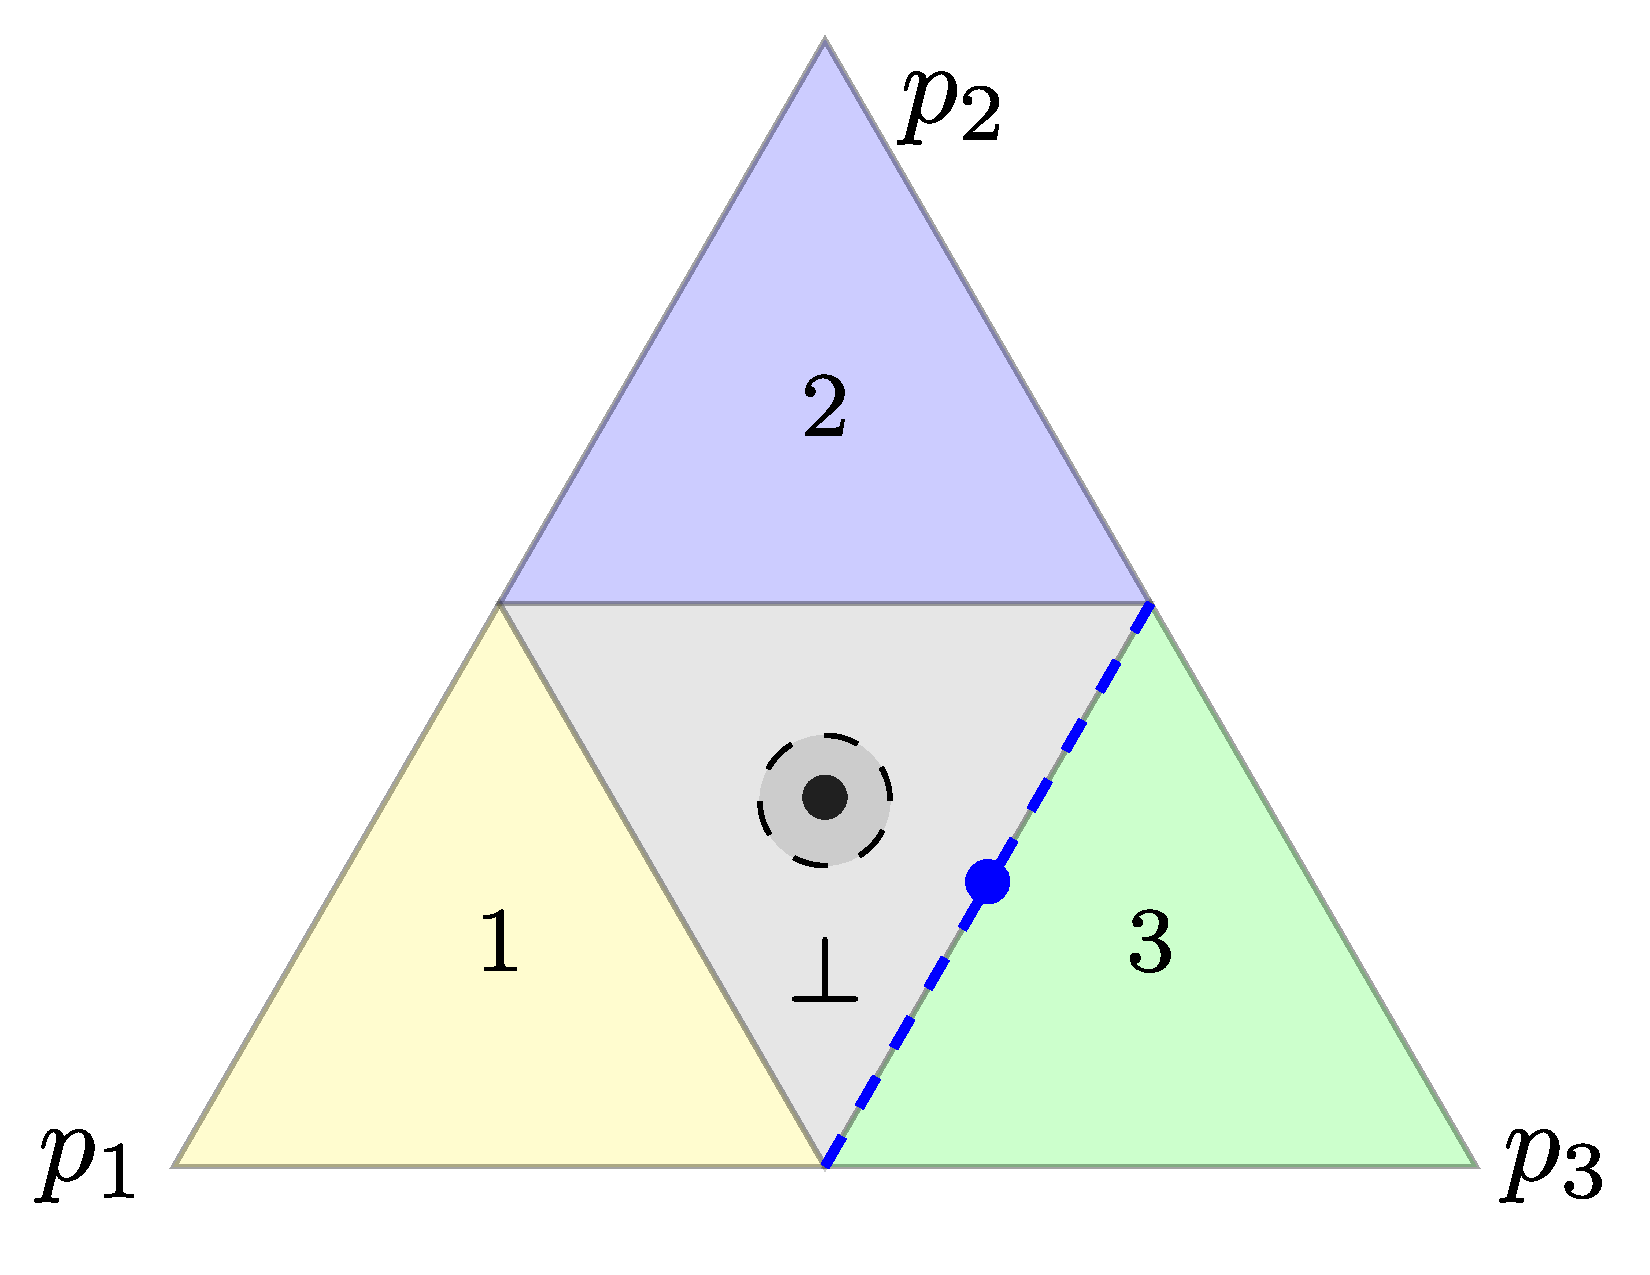
\includegraphics[width=\linewidth]{tikz/fsd-bound.pdf}
	\caption{%Since the uniform distribution is in the relative interior of the simplex and the level set $\gamma_\bot$, 
		$\dim(\Sc_{\gamma_\bot}($\textbullet$)) = 2$ and $\dim(\Sc_{\gamma_\bot}(${\color{blue}\textbullet}$)) = 1$\vspace*{-5pt}}
	\label{fig:fsd-bound}
\end{minipage}
\hfill
\begin{minipage}{0.45\linewidth}
	\centering
	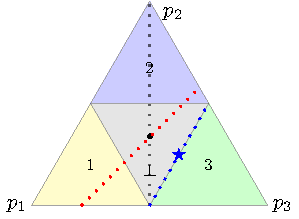
\includegraphics[width=\linewidth]{tikz/flats-bound.pdf}
	\caption{Any $1$-flat $F$ through \textbullet leaves $\gamma_\bot$.
	However, there is a $1$-flat containing {\color{blue} \textbullet} that is a subset of $\gamma_\bot$ and $\gamma_3$.
	}
	\label{fig:flats-bound}
\end{minipage}
\end{figure}

\section{Continuous-valued predictions}\label{sec:contin-consis}

%commented out Jun 1 2020
%Theorem~\ref{thm:consistent-implies-indir-elic} allows us to use convex elicitation complexity as a tool to understand efficiency of consistent convex surrogates for a given property, which is more often what is given in a continuous estimation setting.
%For example, when one wants to learn an $\alpha$-quantile, we start with the property rather than a loss.
%In the literature, pinball loss $L(r,y) = (r-y)(\ones_{r \geq y} - \alpha)$ typically appears without explanation or justification as to why it is relevant in relation to the $\alpha$-quantile.
%Elicitation teaches us why pinball loss is consistent for learning a quantile as the pinball loss elicits the $\alpha$-quantile.
In continuous estimation problems, often one is not given a target loss, but instead a target (conditional) statistic of the data one wishes to estimate, such as the mean or variance.
In this setting, Lemma~\ref{thm:convex-flats-inf-dim} gives lower bounds on the prediction dimension of convex losses with a link to the desired conditional statistic, i.e., the convex elicitation complexity.
In particular,
% following an argument from~\citet{frongillo2018elicitation},
Theorem~\ref{thm:bayes-risk-lower-bound} below yields new bounds on the convex elicitation complexity of statistics which quantify risk or uncertainty such as variance, entropy, or financial risk measures.

These bounds address an open question of~\citet{frongillo2020elicitation}, that of developing a theory of elicitation complexity for with respect to convex-elicitable properties.
The lower bounds of that work are essentially all with respect to identifiable properties, that is, properties $\gamma$ for which there is some $d$ where $\gamma_r$ is a $d$-flat for all $r\in\R$.
In contrast, properties elicited by non-smooth convex losses are generally not identifiable.
For example, the properties elicited by hinge loss and the abstain surrogate are not identifiable, as their level sets are not flats (see Figure~\ref{fig:fsd-bound}).
Establishing a theory of elicitation complexity for convex-elicitable properties therefore seemed to require entirely new ideas.
Surprisingly, we show that the central techniques of~\citet{frongillo2020elicitation} also apply to convex-elicitable properties, via Lemma~\ref{thm:convex-flats-inf-dim}.
In particular, we can recover their main lower bound for the large class of Bayes risks.

% Theorem~\ref{thm:cvx-flats} also addresses one major open question  from~\citet{frongillo2015elicitation,frongillo2018elicitation}\jessiet{which citation?}: \emph{what are lower bounds on convex elicitation complexity?}
% While Theorem~\ref{thm:cvx-flats} is a statement about consistent surrogates, the heart of it is actually about indirect property elicitation.
% Thus, the result also applies to extend previous results~\citep{frongillo2015elicitation,frongillo2018elicitation} to provide new bounds on elicitation complexity for certain classes of properties in Theorem~\ref{thm:bayes-risk-lower-bound}.


% When extending the results of~\cite{frongillo2018elicitation}, we assume a property is identifiable, meaning its level sets are flats.
% \begin{definition}
%   A property $\Gamma:\simplex\to\R$ is \emph{$d$-identifiable} if its level sets are flats of co-dimension at most $d$ intersected with $\simplex$.
%   We write $\iden(\Gamma) = \min\{d \in \mathbb{N} : \Gamma\text{ is $d$-identifiable}\}$.
% \end{definition}

\begin{condition}\label{cond:v-interior}
  There exists $r\in\range\Gamma$, such that $\Gamma_r = \zeros{V}$ is a $d$-flat presented by some $V:\Y\to\reals^d$ such that \raft{I think we only need $\Gamma_r \subseteq \zeros{V}$.  I think I'll update the proof at some point to reflect this, since it actually gets a bit easier to follow.} $0\in\interior\{\E_pV : p\in\P\}$.
\end{condition}

\begin{restatable}{theorem}{bayesrisklowerbound}\label{thm:bayes-risk-lower-bound}\btw{Old version for finite $\Y$ is in the NeurIPS 2020 submission; especially lots more detail on variance / norm / entropy examples}
  Let $\Gamma:\P\to\reals^d$ satisfy Condition~\ref{cond:v-interior} for some $r\in\reals^d$.
  Let $L$ elicit $\Gamma$ such that $\lbar$ is non-constant on $\Gamma_r$.
  Then $\eliccvx(\lbar) \geq d+1$.
\end{restatable}

\begin{proof}[Proof sketch; full proof in Appendix~\ref{app:omitted-proofs}]
  We roughly follow the argument of~\citet[Corollary 7]{frongillo2018elicitation}.
  To indirectly elicit $\lbar$, we must link from a loss $\hat L: \reals^k \times \Y \to \reals$.
  By \citet[Theorem 4]{frongillo2018elicitation}, the property $\hat\Gamma = \prop{\hat L}$ refines $\Gamma$, in the sense that every level set of $\hat\Gamma$ is contained in a level set of $\Gamma$.
  If $\lbar$ is non-constant (the interesting case) on the level set $\Gamma_r$ containing $p$, then $\Gamma_r$ must strictly contain some level set $\hat \Gamma_{\hat r}$ containing $p$.
  But by Theorem 2, there is a flat $\hat{F}$ containing $p$ of codimension at most $k$, yet strictly contained in $\affhull(\Gamma_r)$ of codimension $d$.
  So $k \geq d + 1$.
\end{proof}

We now illustrate the theorem with two important examples: variance and conditional value at risk.
Several other applications from \citet{frongillo2018elicitation}, such as spectral risk measures, entropy, and norms, follow similarly.

\paragraph{Example: Variance.}
As a warm-up, let us see how to show $\eliccvx(\Var)=2$, meaning the lowest dimension of a convex loss to estimate conditional variance is 2.%~\citep{osband1985providing,lambert2018elicitation}.
This lower bound follows from Theorem~\ref{thm:bayes-risk-lower-bound} as the variance is the Bayes risk of squared loss $L(r,y) = (r-y)^2$, which elicits the mean $\Gamma(p) = \E_p Y$.
Interestingly, while intuitively obvious, even this simple result is novel.
In particular, the well-known fact that the variance is not elicitable does not yield a lower bound of 2, as it does not rule out the variance being a link of a real-valued convex-elicitable property; cf.~\citet[Remark 1]{frongillo2018elicitation}.

\begin{corollary}
  \label{cor:variance}
  Let $\P\subseteq\simplex$ for $\Y\subseteq \reals$, such that there exist $p,q,q'\in\P$ with $\E_p Y = \E_q Y \neq \E_{q'} Y$ and $\Var(p) \neq \Var(q)$.
  \raft{Note to self: I think this condition is tight actually: if there is no such triple in $\P$, I think $\eliccvx(\Var) \leq 1$ (i.e., $\Var$ is constant or a function of the mean)}
  Then $\eliccvx(\Var)=2$.
\end{corollary}
\begin{proof}
  For the upper bound, we may elicit the first two moments via the convex loss $L(r,y) = (r_1-y)^2 + (r_2-y^2)^2$, and recover the variance via $\psi(r) = r_2-r_1^2$, giving $\eliccvx(\Var) \leq 2$.
  Now for the lower bound.
  Without loss of generality, $\E_qY < \E_{q'}Y$.
  Let $r = \tfrac 1 2 \E_qY + \tfrac 1 2 \E_{q'}Y$, and define $V:\Y\to\reals, y\mapsto y-r$.
  Then $\zeros{V} = \{p'\in\P \mid \E_{p'}Y=r\} = \Gamma_r$ where $\Gamma:p'\mapsto \E_{p'}Y$ is the mean.
  As $\E_q Y < r < \E_{q'} Y$, we conclude $\E_q V < 0 < \E_{q'} V$.
  We have now satisfied Condition~\ref{cond:v-interior} for $d=1$.
  To apply Theorem~\ref{thm:bayes-risk-lower-bound}, it remains to show that $\Var$ is non-constant on $\Gamma_r$.
  % and the identity $\Var(p') = \E_{p'} Y^2 - (\E_{p'} Y)^2$
  By our assumptions and the definition of $\Var$, we have $\E_p Y^2 \neq \E_q Y^2$.
  Letting $p_1 = \tfrac 1 2 q + \tfrac 1 2 q'$, $p_2 = \tfrac 1 2 p + \tfrac 1 2 q'$, we have $\E_{p_i}Y = r$ for $i\in\{1,2\}$, but $\E_{p_1} Y^2 = \tfrac 1 2 \E_qY^2 + \tfrac 1 2 \E_{q'}Y^2 \neq \tfrac 1 2 \E_pY^2 + \tfrac 1 2 \E_{q'}Y^2 = \E_{p_2}Y^2$.
  As $p_1,p_2$ have the same mean but different second moments, we conclude $\Var(p_1) \neq \Var(p_2)$.
\end{proof}

\paragraph{Example: Conditional Value at Risk.}

\citet{frongillo2018elicitation} observe that one of the most prominent financial risk measures, the conditional value at risk (CVaR), can be expressed as a Bayes risk.
In particular, for $0 < \alpha < 1$, we may define
\begin{align}
  \CVaR_\alpha(p)
  &= \inf_{r\in\reals} \E_p\left\{ \tfrac 1 \alpha(r-Y)\ones_{r\geq Y}- r\right\}~,
  \label{eq:elic-complex-es-3}
\end{align}
which is the Bayes risk of the transformed pinball loss $L_\alpha(r,y) = \tfrac 1 \alpha(r-y)\ones_{r\geq y}-r$.
In turn, $L_\alpha$ elicits the $\alpha$-quantile $q_\alpha(p) = \raf{DEF}$.

\begin{corollary}
  \label{cor:spectral-risks}
  Let $\P$ \raf{four distributions: $p_0,p_1,p_2$ w/ increasing quantiles and $p_1'$ with the same quantile as $p_1$ but different tail}.
  Then $\eliccvx(\CVaR_\alpha) = 2$.
\end{corollary}


\section{Conclusions and future work}\label{sec:conclusions}
In this work, we show that indirect property elicitation can be a powerful necessary condition for the existence of a consistent surrogate loss (Theorem~\ref{thm:consistent-implies-indir-elic}).
Furthermore, we introduce a new lower bound (Corollaries~\ref{cor:Pcodim-flat-single-val-prop} and~\ref{cor:Pcodim-flat-elic-relint-prop}) on the dimension of a consistent convex loss that is generally applicable and extends previous results from both the discrete and continuous estimation settings.

Several important questions remain open.
Particularly for the discrete settings, we would like to know whether one can lift the restriction that surrogates always achieve a minimum; we conjecture positively.
%For continuous settings, it would be especially interesting to extend to the case $\Y=\reals$, which would require a more careful analysis in Theorem~\ref{thm:bayes-risk-lower-bound}.\jessie{Flagging this bc we take care of it I hope}
Of course, we would like to characterize $\ccdim$ and $\eliccvx$ and develop a general framework for constructing surrogates achieving the best possible prediction dimension.
\jessie{for neurips, we had commented out everything below this for space}
One might be able to further tighten these bounds by property elicitation by studying monotonicity and adjacency of level sets.
In discrete predictions, these bounds might also be tightened if the equivalence of convex calibration dimension and embedding dimension of~\citet{finocchiaro2020embedding} is shown; the current embedding dimension bounds are not tight either, but additional structure is imposed by considering the embedding framework.
Moreover, the practical reason why consistency is desired is to ensure the guarantee of empirical risk minimization (ERM) rates; however, the relationship between ERM rates and property elicitation has not been studied.
%Lastly, Theorem~\ref{thm:cvx-flats} relies on Minkowski sums, which have not been clearly defined for infinite $\Y$; we leave this generalization as an open question.

\newpage

%\section*{Broader Impacts}
%\paragraph{Background: surrogate losses and dimension.} There are numerous and growing applications to society, well-known to readers in the field, of supervised machine learning where we learn, from training data pairs $(x,y)$, to predict $y$ from $x$.
%Perhaps the most popular approach to this problem is to train a model to minimize \emph{loss} on the training data, and essentially the only practically-used losses are convex losses on $\reals^d$, generally surrogates for a target loss (such as 0-1 loss for classification) or target statistic to be estimated (such as the conditional median or variance of $y$ given $x$).
%
%This paper may not be relevant to all of these problems, but it is especially relevant where the prediction space of current known consistent surrogates is high-dimensional.
%This can include \emph{structured prediction} problems where the goal is to learn to predict properties like rankings of labels by likelihood, or predicting parse trees from natural language sentences.
%It can also include standard classification tasks where we would like to embed the thousand or more possible labels into a smaller-dimensional prediction space.
%In all of these settings, a lower prediction dimension can translate to improved computation time and reduced sample complexity, allowing algorithms to provide more accurate predictions with less data and compute.
%
%\paragraph{Impact via influence on downstream research.}
%This paper takes a step toward an impactful general program: to understand and design \emph{useful} (i.e. convex, consistent, calibrated, etc.) surrogate losses of low dimensionality.
%The theory in this paper may help practitioners in a number of ways.
%Understanding how to design consistent convex surrogates for different target losses and properties we wish to learn, and when this is impossible, can lead to understanding the tradeoffs that are often made in the current ad-hoc design of surrogates.
%These ad-hoc surrogates are consistent with respect to \emph{some property}, although it may not be the one we wish to elicit, either directly or indirectly.
%As a general prediction task arises, one might be able to use property elicitation to understand what question they are actually answering (in the best case, with sufficient data that matches the real-world data distribution) by minimizing their surrogate loss and how it differs from the question they are actually trying to answer.
%
%Of course, improvements in general machine learning algorithms can be put to many uses in many societal contexts, so a more specific analysis of potential broader impacts appears very difficult to forecast.
%
%
%%% Bo: rewritten Jun 4 8pm
%% A general framework to design consistent convex surrogate losses would have broad impact throughout the applications of machine learning in society.
%% Moreover, in problems such as structural prediction, knowing the lowest possible prediction dimension for a consistent surrogate is crucial for practical performance.
%% Our work advances understanding in both of these questions, and takes an important step toward a general framework which could lead to new surrogates for prediction tasks both new and old.
%
%% Understanding how to design consistent convex surrogates for different target losses and properties we wish to learn, and when this is impossible, can lead to understanding the tradeoffs that are often made in the current ad-hoc design of surrogates.
%% These ad-hoc surrogates are consistent with respect to \emph{some property}, although it may not be the one we wish to elicit, either directly or indirectly.
%% As a general prediction task arises, one might be able to use property elicitation to understand what question they are actually answering (in the best base, with sufficient data that matches the real-world data distribution) by minimizing their surrogate loss and how it differs from the question they are actually trying to answer.

%\begin{ack}
%adam, nishant, nsf grants/fellowship
%\end{ack}

\bibliographystyle{plainnat}
\bibliography{diss,extra}

\newpage
\appendix
\section{A general notion of calibration}\label{app:calibration}
For general settings, we introduce a notion of calibration that is a special case of calibration as introduced by~\cite[Definition 2.7]{steinwart2007compare} and~\citet[Chapter 3]{steinwart2008support}. 
\jessiet{I think we need to be careful how we present this; I'm not sure it's a new definition, though we seem to prove new results about it.}
We will show that in discrete prediction settings, it is equivalent to the more commonplace definition given in Definition~\ref{def:calibrated-finite}.
Therefore, we use this more general definition of calibration when proving statements about the relationship between consistency, calibration, and indirect elicitation.

\begin{definition}[Calibrated]\label{def:calibrated-general}
	A loss $L:\reals^d \times \Y \to \reals$ is \emph{calibrated} with respect to a loss $\ell : \R \times \Y \to \reals$ eliciting the property $\gamma$ \jessie{$\gamma$ isn't used here...?} if there is a link $\psi : \reals^d \to \R$ such that, for all distributions $p \in \P$, there exists a function $\zeta : \reals_+ \to \reals_+$ with $\zeta$ continuous at $0^+$ and $\zeta(0) = 0$ such that for all $u \in \reals^d$, we have
	\begin{equation}\label{eq:calibrated-general}
	\ell( \psi(u); p) - \risk{\ell}(p)  \leq \zeta \left(  \exploss{L}{u}{p} - \risk{L}(p) \right)~.~
	\end{equation}
\end{definition}

Consider the following four conditions: Suppose we are given $\zeta:\reals_+ \to \reals_+$.
\begin{enumerate}
	\item [A] $\zeta$ satisfies $\zeta : 0 \mapsto 0$ and is continuous at $0$.
	\item [B] $\epsilon_m \to 0 \implies \zeta(\epsilon_m) \to 0$.
	\item [C] Given $\zeta:\reals \to \reals_+$, for all $u \in \reals^d$, $R_\ell(\psi(u); p) \leq \zeta(R_L(u;p))$.
	\item [D] For all $p \in \P$ and sequences $\{u_m\}$ so that $R_L(u_m; p) \to 0$, we have $R_\ell(\psi(u_m); p) \to 0$.
\end{enumerate}
The existence of a function $\zeta$ so that $(A \wedge C)$ defines calibration as in Definition~\ref{def:calibrated-general}, and we show $A \iff B$ in Lemma~\ref{lem:continuous-iff-limits}.  
Lemma~\ref{lem:calib-converging-regrets} shows calibration if and only if $D$, which yields a condition equivalent to calibration without dependence the function $\zeta$.

\begin{proposition}
	When $\R$ and $\Y$ are finite, a continuous loss and link $(L, \psi)$ are calibrated with respect to a target loss $\ell$ via Definition~\ref{def:calibrated-general} if and only if they are calibrated via Definition~\ref{def:calibrated-finite}.
  %\btw{Okay if $\Gamma$ is empty}
\end{proposition}
\begin{proof}
$\implies$
	We prove the contrapositive; if $(L, \psi)$ is not calibrated with respect to $\ell$ by Definition~\ref{def:calibrated-finite}, then it is not calibrated via Definition~\ref{def:calibrated-general} either.
	If $(L, \psi)$ are not calibrated with respect to $\ell$ by Definition~\ref{def:calibrated-finite}, then there is a $p \in \P$ so that $\inf_{u : \psi(u) \not \in \gamma(p)} \exploss{L}{u}{p} = \inf_u \exploss{L}{u}{p}$.
	Thus there is a sequence $\{u_m\}$ so that $\lim_{m \to \infty} \psi(u_m) \not \in \gamma(p)$ and $\exploss{L}{u_m}{p} \to \risk{L}(p)$.  
	Now we have $R_L(u_m; p) \to 0$ but $R_\ell(\psi(u_m); p) \not \to 0$, so by Lemma~\ref{lem:calib-converging-regrets}, we contradict calibration by Definition~\ref{def:calibrated-general}.
%	
% Commented out 05.19.2020 for easier proof if Lemma 5 is true.
%	We prove the contrapositive; if $(L, \psi)$ is not calibrated with respect to $\ell$ by Definition~\ref{def:calibrated-finite}, then it is not calibrated via Definition~\ref{def:calibrated-general} either.
%	
%	Suppose there was a distribution $p \in \simplex$ so that $\inf_{u : \psi(u) \not \in \gamma(p)} L(u;p) = \inf_{u} L(u;p)$.
%	There must then be a sequence $\{u_m\} \to u$ so that $\lim_{m \to \infty} \psi(u_m) \not \in \gamma(p)$ and $L(u_m; p) \to \risk{L}(p)$.
%	
%	This consequently implies $R_L(u_m;p) \to 0$ as $L(u_m; p) \to \risk{L}(p)$, but as $\ell(\psi(u_m); p) \not \to \risk{\ell}(p)$ (if it did converge, then we would have $\psi(u_m) \to r \in \gamma(p)$), so $R_\ell(\psi(u_m); p) \not \to 0$.
%	Thus, by Lemma~\ref{lem:calib-converging-regrets}, we have no calibration via Definition~\ref{def:calibrated-general}.  

$\impliedby$
Suppose there was a function $\zeta$ satisfying the bound in Equation~\eqref{eq:calibrated-general} for a fixed distribution $p \in \P$.
Observe the bound in Equation~\eqref{eq:calibration} can be written as $R_L(u,p) > 0$ for all $p \in \simplex$ and $u$ such that $\psi(u)$ is bounded away from $\gamma(p)$. \jessiet{details correct??}

By Equation~\eqref{eq:calibrated-general}, for any sequence $\{u_m\}$ so that $\psi(u_m) \not \to \gamma(p)$, we have must have $\zeta(R_\ell(\psi(u_m), p)) \not \to 0$ as we would otherwise contradict the bound in Equation~\eqref{eq:calibrated-general} since $R_\ell(\psi(u), p) \not \to 0$. 
Therefore $R_L(u_m, p) \not \to 0$; thus, the strict inequality holds.
\end{proof}

The following Lemma shows that conditions $A$ and $B$ are equivalent, so that we can using condition $B$ in lieu of condition $A$ in the proof of Lemma~\ref{lem:calib-converging-regrets}
\begin{lemma}\label{lem:continuous-iff-limits}
	A function $\zeta:\reals \to \reals$ is continuous at $0$ and $\zeta(0) = 0$ if and only if the sequence $\{u_m\} \to 0 \implies \zeta(u_m) \to 0$.
	\jessie{$A \iff B$}
\end{lemma}
\begin{proof}
	$\implies$ Suppose we have a sequence $\{u_m\} \to 0$.
	By continuity, we have $\lim_{u_m \to 0}\zeta(u_m) = \zeta(0) = 0$, so $\zeta(u_m) \to 0$.
	
	$\impliedby$ Suppose $\zeta(0) \neq 0$ but $\zeta$ was continuous at $0$.
	The constant sequence $\{u_m\} = 0$ then converges to $0$, but as $\zeta$ is continuous at $0$, we must have $\lim_{m \to \infty}\zeta(u_m) = \zeta(0) \neq 0$, so $\zeta(u_m) \not \to 0$.
	
	Now suppose $\zeta(0) = 0$ but $\zeta$ was not continuous at $0$.
	There must be a sequence $\{u_m\} \to 0$ so that $\lim_{m \to \infty}\zeta(u_m) \neq \zeta(0) = 0$, so $\zeta(u_m) \not \to 0$.
\end{proof}

Lemma~\ref{lem:calib-converging-regrets} now gives a condition equivalent to calibration without requiring one to already have a function $\zeta$ in mind.
\begin{lemma}\label{lem:calib-converging-regrets}
	A continuous surrogate and link $(L,\psi)$ are calibrated (via definition~\ref{def:calibrated-general}) with respect to $\ell$ if and only if, for all $p \in \P$ and sequences $\{u_m\}$ so that $R_L(u_m; p) \to 0$, we have $R_\ell(\psi(u_m); p) \to 0$.
	\jessie{$(A \wedge C) \iff D$}
\end{lemma}
\begin{proof}
\jessie{$(A \wedge C) \implies D$}
	$\implies$ Take a sequence $\{u_m\}$ so that $R_L(u_m;p) \to 0$.
	Since $\zeta(0) = 0$ and $\zeta$ is continuous at $0$, we have $\zeta(R_L(u_m;p)) \to 0$.
	As the bound from Equation~\eqref{eq:calibrated-general} is satisfied for all $u \in \reals^d$ by assumption, we observe
	\begin{align*}
	\forall m, \; &0 \leq R_\ell(\psi(u_m); p) \leq \zeta(R_L(u_m;p))\\
	\implies &0 \leq \lim_{m \to \infty} R_\ell(\psi(u_m); p) \leq \lim_{m \to \infty} \zeta(R_L(u_m;p)) = 0\\
	\implies &0 = \lim_{m\to\infty} R_\ell(\psi(u_m); p) ~.~
	\end{align*}
	
	
	$\impliedby$ 
\jessie{$D \implies (A \wedge C)$}
	Fix $p \in \P$, and consider $\zeta(c) := \sup_{u: R_L(u,p) \leq c} R_\ell(\psi(u); p)$.  
	We will show $R_L(u_m; p) \to 0 \implies R_\ell(\psi(u_m); p) \to 0$ gives calibration via the function $\zeta$ constructed above. 
	With $\zeta$ as constructed, we observe that the bound in equation~\eqref{eq:calibrated-general} is satisfied for all $u \in \reals^d$ and apply Lemma~\ref{lem:continuous-iff-limits} to observe that if there is a sequence $\{\epsilon_m\} \to 0$ so that $\zeta(\epsilon_m) \not \to 0$, it is because $R_L(u_m, p) \not \to 0 \not\implies R_\ell(\psi(u_m), p) \to 0$.
	

\jessie{D $\implies$ C}
Now, we observe that the bound in Equation~\eqref{eq:calibrated-general} is satisfied for all $u \in \reals^d$ by construction of $\zeta$.
Let $S(v) := \{u' \in \reals^d : R_L(u';p) \leq R_L(v,p) \}$.
Showing $R_\ell(\psi(u);p) \leq \sup_{u' \in S(u)} R_\ell(\psi(u') ; p)$ for all $u \in \reals^d$ gives the condition $C$.
As $u$ is in the space over which the supremum is being taken (as $R_L(u;p) \leq R_L(u;p)$), we then have calibration by definition of the supremum.

\jessie{Not $B$ leads to contradiction of $D$.}
Now suppose there exists a sequence $\{\epsilon_m\} \to 0$ so that $\zeta(\epsilon_m) \not \to 0$.
Consider $S(\epsilon) = \{u \in \reals^d : R_L(u,p) \leq \epsilon\}$.

\begin{align*}
\epsilon_1 \leq \epsilon_2 &\implies S(\epsilon_1) \subseteq S(\epsilon_2)\\
&\implies \zeta(\epsilon_1) \leq \zeta(\epsilon_2)~.~
\end{align*}
Now suppose there exists a sequence $\{u_m\}$ so that $R_L(u_m, p) \to 0$.
Then for all $\epsilon > 0$, there exists a $m' \in \mathbb{N}$ so that $R_L(u_m, p) < \epsilon$ for all $m \geq m'$.
Since this is true for all $\epsilon$, we have $S(\epsilon)$ nonempty for all $\epsilon > 0$, and therefore $\zeta(c)$ is discrete for all $c > 0$.
Now if $\zeta(\epsilon_m) \not \to 0$, it must be because $R_\ell(\psi(u_m), p) \not \to 0$ for some sequence converging to zero surrogate regret, and therefore we contradict the statement $R_L(u_m, p) \to 0 \implies R_\ell(\psi(u_m), p) \to 0$.

Moreover, we argue that such a sequence of $\{u_m\}$ with converging surrogate regret always exists by continuity and boundedness from below of the surrogate loss,
\btw{really just need lower semi-continuity and boundedness from below}
since we can take the constant sequence at the (attained) infimum.
%
%\jessie{$D \implies A$, but actually $\lnot B \wedge C \implies \lnot D$}
%Fix $p \in \simplex$.
%Suppose we have a sequence $\{\epsilon_m\}$ so that $\epsilon_m \to 0$, but $\zeta(\epsilon_m) \not \to 0$.
%If $L$ is continuous over the reals \jessiet{Need this, right?}, then for each $m$, we can construct a subsequence $\{u^j_m\}$ so that $R_L(u^j_m, p) \to \epsilon_m$ for all $m$.
%We can now construct the sequence $\{\epsilon'_m\}$ with $\epsilon'_m = \lim_{j \to \infty} R_L(u^j_m, p)$.
%This sequence converges to $0$, but we have $\lim_{m \to \infty} \zeta(\epsilon'_m) = \lim_{m \to \infty} \lim_{j \to \infty} \zeta(R_L(u^j_m, p)) \not \to 0$. 
%As $R_\ell(\psi(u_m); p) \leq R_L(u_m; p)$ for all $m$, we then have this being true in the limit.
%For this sequence, this then gives a loose bound of $0 \leq \lim_{m\to\infty} R_\ell(\psi(u_m); p) \leq c$. 
%	
\end{proof}

\subsection{Relating calibration, consistency, and indirect elicitation.}
Even with the more general notion of calibration that extends beyond discrete predictions, we still have consistency implying calibration.
\begin{proposition}\label{prop:consistent-implies-calibrated}
	If a loss and link $(L, \psi)$ are consistent with respect to a loss $\ell$, then they are calibrated with respect to $\ell$.
\end{proposition}
\begin{proof}
	We show the contrapositive.
	If $(L, \psi)$ are not calibrated with respect to $\ell$, then there is a sequence $\{u_m\}$ such that $R_L(u_m; p) \to 0$ but $R_\ell(\psi(u_m); p) \not \to 0$ via Lemma~\ref{lem:calib-converging-regrets}.
	Suppose $D \sim \X \times\Y$ has only one $x \in \X$ with $Pr_D(X = x) > 0$ so that $p := D_x$ and $\E_D f(X,Y) = \E_p f(x, Y)$.
	Consider any sequence of functions $\{f_m\} \to f$ with $f_m(x) = u_m$ for all $f_m$.
	Now we have $\E_D L(f_m(X), Y) \to \inf_f \E_D L(f(X), Y)$, but $\E_D \ell(\psi \circ f(X), Y) \not \to \inf_f \E_D \ell(\psi \circ f(X), Y)$, and therefore $(L, \psi)$ is not consistent with respect to $\ell$.
\end{proof}

Moreover, we have calibration implying indirect elicitation.
\begin{lemma}\label{lem:calib-implies-indir}
	If a surrogate and link $(L, \psi)$ are calibrated with respect to a loss $\ell:\R \times\Y \to \reals$, then $L$ indirectly elicits the property $\gamma := \prop{\ell}$.
\end{lemma}
\begin{proof}
	Let $\Gamma$ be the unique property directly elicited by $L$, and fix $p \in \simplex$ with $u$ such that $p \in \Gamma_u$.
	We know such a $u$ exists since $\Gamma(p) \neq \emptyset$.
	As $p \in \Gamma_u$, then $\zeta(\exploss{L}{u}{p} - \risk{L}(p)) = \zeta(0) = 0$, we observe the bound $\ell(\psi(u); p) \leq \risk{\ell}(p)$.
	We also have $\ell(\psi(u); p) \geq \risk{\ell}(p)$ by definition of $\risk{\ell}$, so we must have $\ell(\psi(u);p) = \risk{\ell}(p) = \ell(\gamma(p); p)$, and therefore, $p \in \gamma_{\psi(u)}$.
	Thus, we have $\Gamma_u \subseteq \gamma_{\psi(u)}$, so $L$ indirectly elicits $\gamma$.
\end{proof}

Combining the two results, we can observe the result of Theorem~\ref{thm:consistent-implies-indir-elic} another way: \emph{through calibration}.

\section{Omitted Proofs}\label{app:omitted-proofs}
\subsection{Reconstructing the result of~\citet[Theorem 16]{ramaswamy2016convex}}

A hyperplane weakly separates two sets if its two closed halfspaces respectively contain the two sets.
\begin{lemma}\label{lem:intersect-levelsets}
	If $\gamma: \P \toto \R$ is an elicitable property, then for any pair of predictions $r, r' \in \R$ where $\gamma_r \neq \gamma_{r'}$, there is a hyperplane $H = \{x \in \reals^{\Y} : v \cdot x = 0\}$, for some $v \in \reals^\Y$, that weakly separates $\gamma_r$ and $\gamma_{r'}$ and has $\gamma_r \cap H = \gamma_{r'} \cap H = \gamma_r \cap \gamma_{r'}$.
\end{lemma}
\begin{proof}
	\btw{Bo: the proof holds as written for the case where the level sets have empty intersection.}
	Let $\ell$ elicit $\gamma$.
	Let $v = \ell(r, \cdot) - \ell(r', \cdot)$, interpreted as a nonzero vector in $\reals^\Y$.
	Let $H = \{ q : v \cdot q = 0 \}$.
	If $v \cdot q < 0$, then $r'$ cannot be optimal, so $q \not\in \gamma_{r'}$.
	So $\gamma_{r'} \subseteq \{ q : v \cdot q \geq 0 \}$.
	Symmetrically, $\gamma_r \subseteq \{ q : v \cdot q \leq 0 \}$.
	This is weak separation, and it immediately implies that $\gamma_r \cap \gamma_{r'} \subseteq H$.
	Finally, if and only if $v \cdot q = 0$, i.e. $q \in H$, by definition the expected losses of both reports are the same.
	So $q \in \gamma_r \cap H \iff q \in \gamma_{r'} \cap H$.
	This gives $\gamma_r \cap H = \gamma_{r'} \cap H = \gamma_r \cap \gamma_{r'} \cap H = \gamma_r \cap \gamma_{r'}$.
\end{proof}



\begin{lemma}\label{lem:finite-relint-dim}
  Let the $d$-flat $F\subseteq \P$ (defined over finite $\Y$) contain some $p\in\relint{\P}$.
  Then 
  \begin{enumerate}
  	\item[(i)] $p \in \relint{F}$; 
  	\item[(ii)] $\dim(\Scr_F(p)) \geq \dim(\spn(\P - \{p\})) - d$.
  \end{enumerate}
\end{lemma}
\jessiet{Bo had a good point that $\spn(F_p)$ is probably easier to understand, instead of having an extra layer of notation in there.  Do we want to stick with $\Scr_F(p)$ or $\spn(F_p)$?}
\begin{proof}
  %\raf{Moved; see margin comment:  for the function $W : \Y \to \reals^d$ such that $F = \zeros{W}$.  (Such a function must exist by $F$ being a $d$-flat.)}
  
  As $F$ is a $d$-flat, we have some $W:\Y \to \reals^d$ such that $F = \zeros{W}$.
  Throughout, given a point (typically a distribution) $p$ and convex set $P$, we define $P_p := P - \{p\}$.
  Define $T_W:\spn(\P_p)\to\reals^d, v\mapsto \E_v W$.
  
  (i)
  Since $p \in \relint{\P}$, for all $q \in \P$, there is some small enough $\epsilon > 0 $ so that for all $\alpha \in (-\epsilon,\epsilon)$, the point $q_\alpha := p - \alpha(q - p)$ is still in $\P$.
  In particular, for $q \in F$, we claim $q_\alpha \in F$.
  %\raft{$V$ comes out of nowhere here, and then in the next bullet you introduce $W$ for the same thing. Better to do all that before both bullets. ``As $F$ is a $d$-flat, we have some $W$... $F=\zeros{W}$''.  Also, okay to just write $\E_p W$ not $\E_p W(Y)$, since technically $W$ is a random variable.}
  As $p,q \in F$, we have $\E_pW = \E_qW = \vec 0$.
  By linearity of expectation, we then have $\E_{q_\alpha} W = \vec 0$.
  % (Y) = \E_p V(Y) - \alpha(\E_q V(Y) - \E_p V(Y)) = \vec 0 - \alpha(\vec 0 - \vec 0) = \vec 0$.
  This implies $q_\alpha \in F$, and therefore $p \in \relint{F}$.
  
  (ii)
  We first show $\spn(F_p) = \Scr_F(p)$.
  First, take $v \in \Scr_F(p)$, and take $\epsilon_0$ as in the definition.
  For $\epsilon = \epsilon_0 / 2$, we then have $p + \epsilon v \in F \implies \epsilon v \in F_p$, and therefore, $v \in \spn(F_p)$.  
  Now take $v \in \spn(F_p)$.
  Since $p \in \relint{F}$ (i), we have $\vec 0 \in \relint{F_p}$.
  Therefore there is an $\epsilon_0 > 0$ so that $\epsilon v \in F_p$ for all $\epsilon \in (-\epsilon_0, \epsilon_0)$ by convexity of $F$.
  Therefore, $v \in \Scr_F(p)$, and the equality follows.
  
  We now show $\Scr_F(p) = \ker(T_W)$.
%  Let $v \in \ker(T_W)$. % = \{v \in \spn(\P_p) : T_W(v) = \vec 0\}$.
%  From (i), as $p \in \relint{\P}$, we have $\vec 0 \in \relint{F_p}$.
%  Thus there is some $\epsilon > 0$ so that $\epsilon v \in F_p$ and $-\epsilon v \in F_p$.
%  As $\epsilon v \in F_p$, and $v$ is a scalar multiple of it, we additionally conclude $v \in \spn(F_p)$.
%  Moreover, we have $\pm \epsilon v \in \ker(T_W)$ by linearity of expectation, so $v \in \relint{\ker(T_W)}$.
%  Hence, $\spn(F_p) = \ker(T_W)$.\jessie{Right?}\raf{Why? Hint: you want to show $v$ is in the span of $F_p$; in fact, it's a scalar multiple of something in $F_p$.}
%  
%  more up to date than above; commented out 1.25.21
%  Let $v \in \Scr_F(p)$.
%  Then there is some $\alpha$ so that $\alpha v \in F_p$.
%  This means $\E_{\alpha v} W = \vec 0$, which in turn implies $\alpha v \in \ker(T_W)$.
%  By linearity of expectation, we additionally have $v \in \ker(T_W)$.
%  Thus, $\Scr_F(p) \subseteq \ker(T_W)$.
%
  Observe that $\Scr_F(p) \subseteq \ker(T_W)$ follows trivially from the definitions of the two functions. 
  Now let $v \in \ker(T_W)$, and $v' \in F_p$.
  This means $\E_v W = \vec 0$, so it suffices to show $v = c v' \in F_p$, thus showing $v \in \Scr_F(p)$.
  Since $p \in \relint{\P}$, we must have $\vec 0 \in \relint{F_p}$, so we know there is some small enough $\epsilon > 0$ so that $-\alpha v' \in F_p$ for $\alpha \in (-\epsilon, \epsilon)$.
  Take $c = -\alpha$, and we conclude $v \in \Scr_F(p)$.
  Therefore, $\ker(T_W) = \Scr_F(p)$.
  
  As $\Y$ is a finite set, $\spn(\P_p)$ is a finite-dimensional vector space.
  The rank-nullity theorem states $\dim(\im(T_W)) + \dim(\ker(T_W)) = \dim(\spn(\P_p))$.
  As $\dim(\im(T_W)) \leq d$, and we have shown above that $\Scr_F(p) = \ker(T_W)$, the conclusion follows.
  % 
  %	Now let $v \in \ker(T_W) = \{v \in \spn(\P_p) : T_W(v) = \vec 0\}$.
  %	There must exist an $\epsilon > 0$ so that $\epsilon v \in F_p$ and $-\epsilon v \in F_p$ $p \in \relint{\P}$ implies $\vec 0 \in \relint{F_p}$ by (1.).
  %	Moreover, we have $\pm \epsilon v \in \ker(T_W)$ by linearity of expectation, so $v \in \relint{\ker(T_W)}$.
  %	This allows us to conclude $\spn(F_p) = \ker(T_W)$.\jessie{Right?}
  %	
  %	We want to show $F_p = \P_p \cap \ker(T_W)$, then derive the result from there. \jessie{I don't see why this is necessary.}
  %	
  %	In order to see this, consider $v \in F_p \iff v + p \in F$, and similarly for $\P_p$.
  %	Now, as $F \subseteq \P$ by construction, we have $F_p \subseteq \P_p$, and since $\spn(F_p) = \ker(T_W)$, we additionally have $F_p \subseteq \ker(T_W)$, yielding $F_p \subseteq \P_p \cap \ker(T_W)$.
  %	Now consider $v \in \P_p \cap \ker(T_W)$; we know that $\E_v W = \vec 0$, and therefore, $\E_{q} W = \vec 0$, so $v \in F_p$, thus $F_p = \P_p \cap \ker(T_W)$.
  %	
  %	Since $\spn(F_p) = \ker(T_W)$, we have $\dim(\spn(F_p)) = \dim(\ker(T_W)) \geq \dim(\spn(\P_p)) - d$ by \jessie{isomorphism theorem} since $F_p = \ker(T_W) \cap \P_p$. \jessie{??}
\end{proof}

% Commented out 01.26.2021 - Jessie to simplify proof of \hariresult
%\begin{lemma}\label{lem:Fp-subset-feasible-subset}
%Suppose we are given $p \in \relint{\P}$, property $\gamma: \P \toto \R$, and report $r \in \gamma(p)$.
%If $\gamma$ is indirectly elicited by a convex $L \in \L_d$, then there is a $d$-flat $F$ such that $p \in F$ and $F_p \subseteq \Sc_{\gamma_r}(p)$.	
%\end{lemma}
%\begin{proof}
%	Construct $F$ as in Lemma~\ref{thm:convex-flats-inf-dim}; $F$ is a $d$-flat, contains $p$, and we have $F \subseteq \gamma_r$.
%	We aim to show $v \in F_p \implies v \in \Sc_{\gamma_r}(p)$.
%	By Lemma~\ref{lem:finite-relint-dim}(i), we know $p \in \relint{F}$, and therefore, $\vec 0 \in \relint{F_p}$.
%	Consider $v \in F_p$.
%	By $F_p$ being convex and $\vec 0 \in \relint{F_p}$, we know there exists an $\alpha > 0$ so that $-\alpha v \in F_p$.
%	This implies $p - \alpha v \in F \implies p - \alpha v \in \gamma_r \implies v \in \Sc_{\gamma_r}(p)$ since $F$ and $\Sc_{\gamma_r}(p)$ are convex and $F \subseteq \gamma_r$.
%	This yields the desired result, $F_p \subseteq \Sc_{\gamma_r}(p)$.\raft{It feels weird how redundant this is from the argument in the 1st paragraph of (ii) above, but okay for now.}
%\end{proof}

\begin{lemma}\label{lem:set-valued-prop-flats}
	Suppose we are given an elicitable property $\gamma : \P \toto \R$, where $\Y$ is finite, and distribution $p \in \relint\P$ such that $p \in \gamma_r \cap \gamma_{r'}$ for $r,r' \in \R$.
	Then for any flat $F$ containing $p$, $F \subseteq \gamma_r \iff F \subseteq \gamma_{r'}$.
\end{lemma}
\begin{proof}
	If $\gamma_r = \gamma_{r'}$, we are done.
	Otherwise, Lemma \ref{lem:intersect-levelsets} gives a hyperplane $H = \{ x \in \reals^\Y : v \cdot x = 0\}$ and a guarantee that $\gamma_r \subseteq \{ q \in \simplex : v \cdot q \leq 0\}$, while $\gamma_{r'} \subseteq \{ q \in \simplex : v \cdot q \geq 0 \}$, and finally $\gamma_r \cap \gamma_{r'} \subseteq H$.

Suppose $F \subseteq \gamma_r$; we wish to show $F \subseteq \gamma_{r'}$.
Let $q \in F$.
By Lemma~\ref{lem:finite-relint-dim}(i), we have $p \in \relint{F}$, so there exists $\epsilon > 0$ so that $q' = p - \epsilon (q-p) \in F$.

Now, suppose for contradiction that $q \not\in \gamma_{r'}$.\jessiet{I think this can be made more concise, but is clearest this way; it's a bit tricky with the movement between discussing flats and hyperplanes and being subsets of level sets, etc.}
Then $v \cdot q < 0$: containment in $\gamma_r$ gives $v \cdot q \leq 0$, and if $v \cdot q = 0$ then $q \in \gamma_r \cap H \implies q \in \gamma_{r'}$, a contradiction.
But, noting that $p \in H$, we have $v \cdot q' = -\epsilon (v \cdot q) > 0$, so $q'$ is not in $\gamma_{r}$.
This contradicts the assumption $F \subseteq \gamma_r$.
Therefore, we must have $q \in \gamma_{r'}$, so we have shown $F \subseteq \gamma_{r'}$.
Because $r$ and $r'$ were completely symmetric, this completes the proof.
%
% %commented out 01.22.2021 - Jessie; incorporating Lemma that says p in relint(F)	
%	Suppose $F \subseteq \gamma_r$.
%	We show $F \subseteq \gamma_{r'}$.
%	Let $q \in F$.
%	We claim that for small enough $\epsilon$, the point $q' = p - \epsilon (q-p)$ is in $F$ as well.
%	Containment in $F$ follows because both $p$ and $q$ are in $F$ and it is a flat, while containment in $\P$ follows because $p \in \relint\P$. \jessie{Does $\relint{F}$ actually come in here?}
%	
%	Now, suppose for contradiction that $q \not\in \gamma_{r'}$.
%	Then $v \cdot q < 0$: containment in $\gamma_r$ gives $v \cdot q \leq 0$, and if $v \cdot q = 0$ then $q \in \gamma_r \cap H \implies q \in \gamma_{r'}$, a contradiction.
%	But, noting that $p \in H$, we have $v \cdot q' = -\epsilon (v \cdot q) > 0$, so $q'$ is not in $\gamma_{r}$.
%	This contradicts the assumption $F \subseteq \gamma_r$.
%	Therefore, we must have $q \in \gamma_{r'}$, so we have shown $F \subseteq \gamma_{r'}$.
%	Because $r$ and $r'$ were completely symmetric, this completes the proof.
\end{proof}


%\begin{lemma}\label{lem:feas-sub-is-a-flat}
%	Suppose we have the discrete elicitable property $\gamma$ and distribution $p \in \relint{\simplex}$ with $r \in \gamma(p)$.
%	If $F$ is a flat so that $p \in F \subseteq \gamma_r$, then $F' := F - \{p\}$ is contained in $\Sc_{\gamma_r}(p)$.
%	%  \raf{I think you want $p$ in the interior of the simplex for now}
%\end{lemma}
%\begin{proof} \jessie{Better to combine; not currently using this}
%	We aim to show $v \in F' \implies v \in \Sc_{\gamma_r}(p)$.
%	First, observe $v \in F' \iff p + v \in F$.
%	As $p \in \relint{\simplex}$, by Lemma~\ref{lem:finite-relint-dim}, we additionally have $p \in \relint{F}$, and in turn $\vec 0 \in \relint{F'}$.
%	
%	Suppose $v \in F'$, and since $p \in \relint{F}$, there is an $\epsilon > 0$ so that for all $\alpha \in (-\epsilon, \epsilon)$, we have $p + \alpha v \in F \implies p + \alpha v \in \gamma_r$, since $F$ is convex.%, as are level sets of elicitable properties~\cite{lambert2009eliciting}.
%	The result follows by applying the definition of Feasible Subspaces.
%	%By definition of $\Sc_{\gamma_r}(p)$, there is then an $\epsilon$ satisfying the requirement for $v \in \Sc_{\gamma_r}(p)$, so we can conclude $v \in \Sc_{\gamma_r}(p)$, yielding the desired result.
%	
%% %commented out 01.21.2021 - Jessie
%%	\jessie{Revisit this proof}
%%	Observe $F-p$ is a subspace as it is a linear shift of $F$, which is a linear subspace by definition of a flat and the fact that it contains $\vec 0$ (since $F$ contains $p$, which we subtract from).
%%	Now consider $v \in F - p$.
%%	Since $p \in \relint{\P}$, there is an open ball of radius $\epsilon$ in the span of $\P$ so that for all $q \in B(p, \epsilon)$, we have $q \in \P$.
%%	In particular, take $\alpha = \epsilon / 2$, and we observe $p \pm \alpha v \in B(p, \epsilon)$, and therefore $p \pm \alpha v \in \P$.
%%	Moreover, by the assumption $v \in F - p$, we also have $p \pm \alpha v \in \gamma_r$. 
%%	Since level sets of elicitable properties are convex (\citep{lambert2009eliciting}) this is true for all $\alpha' \in [0,\alpha]$.
%%	Therefore, we observe $v \in S_{\gamma_r}(p)$, so $F-p \subseteq S_{\gamma_r}(p)$.
%\end{proof}


\newcommand{\simplexp}{\Delta_{\Y'}}

%commenting out 01.25.2021 since we really just need one direction.
%\begin{lemma}\label{lem:p-boundary-fsd}
%	For any $p \in \P$ and $r$ such that $p \in \gamma_r$, take $\Y' := \supp(p)$.
%	Define $\gamma' : \P \toto \R$ with $\gamma' : q \mapsto \gamma(q) \cap \simplexp$.
%	Then $\Sc_{\gamma_r}(p) = \Sc_{\gamma'_r}(p)$.
%\end{lemma}
%\begin{proof}
%	Consider the ambient space of both $\Sc_{\gamma_r}(p)$ and $\Sc_{\gamma'_r}(p)$ is $\reals^\Y$.
%	We trivially have $\dim(\Sc_{\gamma_r}(p)) \geq \dim(\Sc_{\gamma'_r}(p))$ since $\gamma'$ is simply $\gamma$ projected down to an affine subspace of $\reals^\Y$.
%	
%	Now to see $\dim(\Sc_{\gamma_r}(p)) \leq \dim(\Sc_{\gamma'_r}(p))$, it suffices to show subset inclusion.
%	Take some $v \not \in \Sc_{\gamma'_r}(p)$.
%	Observe that $\gamma'_r = \gamma_r \cap \simplexp$, so if $q^\pm := p \pm \epsilon v \not \in \gamma'_r$ for all $\epsilon > 0$ (i.e. $p \not \in \relint{\simplexp}$), it is either because one of $q^+$ or $q^-$ is not in $\gamma_r$ or because either $q^\pm \not \in \simplexp$.
%	The first case can be seen easily by the definition of $\gamma'$, and the latter can be seen because leaving $\simplexp$ means one of $q^\pm$ also is not in $\P$, and therefore not in $\gamma_r$ as $\gamma_r \subseteq \P$.
%	Thus $\Sc_{\gamma_r}(p) = \Sc_{\gamma'_r}(p)$.
%	%commented out 05.26.2020
%	%	For simplicity, consider $\epsilon = \epsilon_0 / 2$.
%	%	Consider $P := \spn(\{e_y : y \in \supp(p) \})$.
%	%	\begin{align*}
%	%	\dim(\Sc'_{\gamma_r}(p)) &= \dim(\Sc_{\gamma_r}(p)) + \dim(P) - \dim(\Sc_{\gamma_r}(p) + P)
%	%	\end{align*}
%	%	If $\dim(P) = \dim(\Sc_{\gamma_r}(p) + P)$, the claim holds.
%	%	Be definition of $P$, we know $\dim(P) = \|p\|_0$, so we can show $\dim(\Sc_{\gamma_r}(p) + P) = \|p\|_0$.		
%	%	One way to do this is to show $\Sc_{\gamma_r}(p) \subseteq P$.
%	%	
%	%	Suppose there was some $v \not\in P$ such that $v \in \Sc_{\gamma_r}(p)$.
%	%	That means there is some $i$ so that $i \not \in \supp(p)$ (i.e. $p_i = 0$) but $v_i \neq 0$. \jessiet{Check this line.}
%	%	However, if $v \in \Sc_{\gamma_r}(p)$, then there is some $\epsilon_0 > 0$ so that $p + \epsilon v$ and $p - \epsilon v \in \gamma_r \subseteq \simplex$ for all $\epsilon \in (0, \epsilon_0)$.
%	%	For simplicity, consider $\epsilon = \epsilon_0 / 2$.
%	%	Since $p_i = 0$, this gives $(p+\epsilon v)_i = (\epsilon v)_i$, and likewise for $(p - \epsilon v)_i$.
%	%	As neither $\epsilon$ nor $v_i$ are $0$, one of these terms must be negative, and therefore not in the simplex.
%	%	As $\gamma_r \subseteq \simplex$, we then have $v \not \in \Sc_{\gamma_r}(p)$.
%	%	Therefore, $\Sc_{\gamma_r}(p) \subseteq P$, and $\dim(\Sc_{\gamma_r}(p) + P) = \dim(P) = \|p\|_0$.
%\end{proof}

\hariresult*
\begin{proof}
	Let $L : \reals^d \times \Y \to \reals$ elicit $\Gamma$ be a calibrated surrogate for $\ell$, and consider $\Y^{\proj(q)} := \supp(q)$ for any $q \in \simplex$ and what happens when we restrict $L$ and $\ell$ to only the outcomes in $\Y^{\proj(q)}$.
	Take $L^{\proj(q)} := L|_{\Y^{\proj(q)}}$ and $\ell^{\proj(q)} := \ell|_{\Y^{\proj(q)}}$.
	In particular, take $\Y' = \Y^{\proj(p)}, L' = L^{\proj(p)}$, and $\ell' = \ell^{\proj(p)}$. 
	By calibration, we have $L$ indirectly eliciting $\gamma$.
	
	
	Now, observe $L'$ (eliciting $\Gamma'$) indirectly elicits $\gamma' := \prop[\simplexp]{\ell'}$ since, for all $q \in \simplex$, taking $P(q) \in \simplexp$ to be $q$\jessiet{Rename this projection} projected onto $\simplexp$ by removing $0$ entries of $q$, and letting $p' = P(p)$, we have $p' \in \Gamma'_u \implies p' \in \gamma'_{\psi(u)}$.
	Moreover, $\Gamma(p) = \Gamma'(p')$ and $\gamma(p) = \gamma'(p')$.
	This same observation can be used to observe that $L'$ is also calibrated with respect to $\ell'$ as the calibration bound holds for all $q \in \simplex$, and therefore for all $P(q)$ by equality of $\gamma(q) = \gamma^{\proj(q)}(P(q))$.
	
	As $L'$ is calibrated (and consistent) with respect to $\ell'$ and indirectly elicits $\gamma' := \prop[\simplexp]{\ell'}$, then by Corollary~\ref{cor:Pcodim-flat-elic-relint-prop}, we know there exists a $d$-flat $F$ with $p' \in F \subseteq \gamma'_r$.
	Taking $\P = \simplexp$, we know $p' \in \relint{\simplexp}$ by construction, so we can apply Lemma~\ref{lem:finite-relint-dim}(ii), which gives $\dim(\Scr_F(p')) \geq \dim(\spn(\simplexp - \{p\})) =  \dim(\affhull(\simplexp)) - d = \|p\|_0 - 1-d$.\footnote{To construct this second equality, observe $\dim(\spn(\simplexp - \{p\})) \leq \dim(\affhull(\simplexp))$ by using the standard basis for affine hull of the simplex.  For $\dim(\spn(\simplexp - \{p\})) \geq \dim(\affhull(\simplexp))$, observe that the uniform distribution on $\simplexp$ has full support and therefore requires $\|p\|_0 - 1$ elements in its basis.}
	%which gives $\dim(\Scr_F(p')) \geq \dim(\spn(\P_{p'})) - d$.
	%Since $\P = \simplexp$ and $p' \in \relint{\simplexp}$, we have $\dim(\spn(\P_{p'})) = \dim(\affhull(\simplexp)) = \|p\|_0 - 1$. \jessie{How to get rid of sub p notation here?}
	%Therefore, $\dim(\spn(F_p)) \geq \|p\|_0 - 1 - d$
	\raft{Might be nicer on the reader to add one more step for $\|p\|_0$. Also, I just realized we are using $p\in\simplex$ here, but then $p$ can't be in $F\subseteq\Delta_{\Y'}$ ($p$ is an $n$-vector). So maybe we need a $p'$ too.\jessie{Is this better now?  Slash can we remove this comment?}}
	Additionally, $\Scr_F(p') \subseteq \Sc_{\gamma'_r}(p')$ by subset inclusion of the sets themselves.
	Moreover, we have $\Sc_{\gamma_r}(p) \supseteq \Sc_{\gamma'_r}(p')$ trivially.
	%By Lemma~\ref{lem:p-boundary-fsd}, we additionally have $\Sc_{\gamma_r}(p) = \Sc_{\gamma'_r}(p')$.
	Chaining these results, we obtain 
	\begin{align*}
	\dim(\Sc_{\gamma_r}(p)) &\geq \dim(\Sc_{\gamma'_r}(p'))  \geq \dim(\Scr_F(p')) \geq \|p\|_0 - 1 - d~.~
	\end{align*}
%
%	this yields the bound $\dim(\spn(F-\{p\})) \geq \|p\|_0 - 1 - d$.
%	Chaining inequalities, we then have $\dim(\Sc_{\gamma'_r}(p)) \geq \dim(\spn(F - \{p\})) \geq \|p\|_0 - d- 1$ as Lemma~\ref{lem:feas-sub-is-a-flat} states $F - \{p\}$ is a subspace of $\Sc_{\gamma'_r}(p)$.
%	Lemma~\ref{lem:p-boundary-fsd} then states $\dim(\Sc_{\gamma'_r}(p)) = \dim(\Sc_{\gamma_r}(p))$, and from there we observe the result.
	%
	%
	%\old version of the proof from NeurIPS or before - 01.21.2021
	%	First, for intuition, consider $p \in \relint{\simplex}$. 
	%	Theorem~\ref{thm:cvx-flats} implies that there exists a flat $F'$ of affine dimension at least $n-d-1$.
	%	Lemma~\ref{lem:feas-sub-is-a-flat} then says that $\dim(\Sc_{\gamma_r}(p)) \geq \dim(F') \geq n-d-1 \implies d \geq n - \dim(\Sc_{\gamma_r}(p)) - 1$.
	%
	%	
	%	If we can show that $L' := L|_{\Y'}$ is calibrated with respect to $\ell' := \R \times \Y' \to \reals$ with $\ell(r,y) = \ell'(r,y)$ for all $r \in \R$ and $y \in \Y'$ and indirectly elicits $\gamma' := \prop{\ell'}$, then we observe the existence of a flat $F^*$ of codimension $d$ (in $\reals^{\Y'}$) so that $\dim(F^*) = \|p\|_0 - d - 1$ by Theorem~\ref{thm:cvx-flats}.
	%	Then we can use Lemma~\ref{lem:p-boundary-fsd} to observe $\dim(\Sc_{\gamma'_r}(p)) = \dim(\Sc_{\gamma_r}(p))$, and thus the result holds.
	%	
	%	Now to see that $L'$ is calibrated with respect to $\ell'$, consider that $\gamma(p) = \gamma'(p)$ for all $p \in \Delta^{\Y'}$,
	%	\begin{align*}
	%		\forall p \in \Delta_{\Y'}:  \inf_{u \in \reals^d : \psi(u) \not \in \gamma'(p)} L'(u;p) = \inf_{u \in \reals^d : \psi(u) \not \in \gamma(p)} L(u;p) > \inf_{u \in \reals^d} L(u;p) = \inf_{u \in \reals^d} L'(u;p)~.~
	%	\end{align*}
	%	Therefore, we have $L'$ calibrated with respect to $\ell'$.
	%
	%	Moreover, we want to show $L'$ indirectly elicits $\gamma'$ so we can apply Theorem~\ref{thm:cvx-flats}.
	%	First, observe that $L'$ elicits $\Gamma' : p \mapsto \Gamma(p)$ for all $p \in \Delta_{\Y'}$ 
	%	For all $p \in \simplex$, we have $u \in \Gamma(p) \implies \psi(u) \in \gamma(p)$.
	%	As $\Delta_{\Y'} \subseteq \simplex$, this is in particular true for all $p \in \Delta_{\Y'}$.
	%	Therefore, for all $p \in \Delta_{\Y'}$, we have $\Gamma'_u = \Gamma_u \cap \Delta_{\Y'} \subseteq \gamma_{\psi(u)} \cap \Delta_{\Y'} = \gamma'_{\psi(u)}$, and thus $L'$ indirectly elicits $\gamma'$.
\end{proof}

\subsection{Proof of Theorem~\ref{thm:bayes-risk-lower-bound}}

\begin{lemma}[\citep{frongillo2018elicitation}]
	\label{lem:elic-complex-bayes-concave}
	Suppose the loss $L$ elicits a single-valued property $\Gamma:\simplex\toto\R$.
	Let $\lbar$ be the Bayes risk of $L$.
	Then for any $p,p'\in\simplex$ with $\Gamma(p)\neq\Gamma(p')$, we have $\lbar(\lambda p + (1-\lambda) p') > \lambda \lbar(p) + (1-\lambda) \lbar(p')$ for all $\lambda\in(0,1)$.
\end{lemma}

% \begin{lemma}\label{lem:affhull-interior}
%   \raf{Skip this...}
%   Let $C\subseteq\reals^m$ be convex with nonempty interior $\mathring C$.
%   Then for any flat $F\subseteq\reals^m$ with $F\cap\mathring C \neq \emptyset$, we have $\affhull(F\cap C) = F$.
% \end{lemma}
% \begin{proof}
%   As $\affhull(F) = F$ and $F\cap C\subseteq F$, the inclusion $\affhull(F\cap C) \subseteq F$ is clear.
%   For the reverse, let $p\in F\cap\mathring C$ and let $B\subseteq C$ be an open set containing $p$.
%   For any $q\in F$, we thus have $q' = p + \epsilon (q-p) \in B$ for sufficiently small $\epsilon > 0$.
%   As $q' = (1-\epsilon) p + \epsilon q$, we have $q' \in \affhull(F)\cap C = F\cap C$.
%   As $q = (1-1/\epsilon) p + (1/\epsilon) q'$, we thus have $q\in\affhull(F\cap C)$.
% \end{proof}

\begin{lemma}\label{lem:affhull-relint}
	Let $C\subseteq\reals^m$ be convex.
	Then for any affine subspace $F\subseteq\affhull(C)$ with $F\cap\relint C \neq \emptyset$, we have $\affhull(F\cap C) = F$.
\end{lemma}
\begin{proof}
	As $\affhull(F) = F$ and $F\cap C\subseteq F$, the inclusion $\affhull(F\cap C) \subseteq F$ is clear.
	For the reverse, let $p\in F\cap\relint C$ and let $B\subseteq C$ be a relatively open set containing $p$.
	For any $q\in F \subseteq \affhull(C)$, we thus have $q' = p + \epsilon (q-p) \in B$ for sufficiently small $\epsilon > 0$.
%	\bo{How does this follow exactly from B relatively open?}
	As $q' = (1-\epsilon) p + \epsilon q$, we have $q' \in \affhull(F)\cap C = F\cap C$.
	As $q = (1-1/\epsilon) p + (1/\epsilon) q'$, we thus have $q\in\affhull(F\cap C)$.
\end{proof}

\bayesrisklowerbound*
\begin{proof}
	Suppose that we have some convex loss $\hat L:\reals^k\times\Y\to\reals$ eliciting a property $\hat\Gamma:\simplex\to\reals^k$, and link $\psi : \reals^k \to \reals$ such that $\lbar = \psi \circ \hat\Gamma$.
	% The condition $\iden(\Gamma)=d$ implies the existence of some level set $\Gamma_r$ such that $\codim(\affhull(\Gamma_r)) \geq d$; otherwise, taking $F_r = \affhull(\Gamma_r)$ for all reports $r\in\reals^d$, we would have $\codim(F_r) \leq d-1$ and $\Gamma_r = F_r \cap \simplex$, implying $\iden(\Gamma)\leq d-1$.
	The proof of \citet[Theorem 4]{frongillo2018elicitation} argues that $\hat\Gamma$ must refine $\Gamma$, in the sense that every level set of $\hat\Gamma$ is contained in a level set of $\Gamma$; for completeness we give the argument here.
	Suppose for a contradiction that we have $p,p'$ with $\hat\Gamma(p)=\hat\Gamma(p')$ but $\Gamma(p) \neq \Gamma(p')$.
	As $\lbar = \psi \circ \hat\Gamma$, we also have $\lbar(p) = \lbar(p')$.
	Letting $p'' = \tfrac 1 2 p +  \tfrac 1 2 p'$, Lemma~\ref{lem:elic-complex-bayes-concave} would then give us $\lbar(p'') >  \tfrac 1 2 \lbar(p) +  \tfrac 1 2 \lbar(p') = \lbar(p)$.
	By \citet{osband1985providing}, the level sets $\hat\Gamma_{\hat r}$ are convex, giving $\hat\Gamma(p'') = \hat\Gamma(p)$, which would imply $\lbar(p'')=\lbar(p)$, contradicting $\lbar = \psi \circ \hat\Gamma$.
	We conclude $\hat\Gamma$ must refine $\Gamma$, and thus $\hat L$ actually indirectly elicits $\Gamma$ through some other link function.
	% The proof of \cite[Theorem 4]{frongillo2018elicitation} argues that $\hat\Gamma$ must refine $\Gamma$, in the sense that for all $\hat r \in \hat\Gamma(\simplex)$ we have $\hat\Gamma_{\hat r} \subseteq \Gamma_r$ for some $r\in\reals^k$.
	
	In particular, we have $p \in \hat \Gamma_{\hat r} \subseteq \Gamma_r$ for some $\hat r, r$.
	By Theorem~\ref{thm:cvx-flats}, there is a flat $\hat F \subseteq \affhull(\simplex)$ containing $p$ such that $\codim(\hat F) \leq k$ and $S := \hat F \cap \simplex \subseteq \hat\Gamma_{\hat r} \subseteq \Gamma_r$.
	% Let $F' = \hat F \cap \affhull(\simplex)$, and observe the following: $p\in F'\cap\relint\simplex$, $F' \subseteq \affhull(\simplex)$, $S=F'\cap\simplex\subseteq\Gamma_r$, and $\codim(F') \leq k+1$.
	% the next \hat Fs used to be F's
	As $p\in \hat F\cap\relint\simplex$, Lemma~\ref{lem:affhull-relint} gives $\affhull(S) = \hat F$.
	Let $F = \affhull(\Gamma_r)$ and recall $\codim(F)=d$.
	Now as $S \subseteq \Gamma_r$, we also have $\hat F = \affhull(S) \subseteq \affhull(\Gamma_r) = F$,
	implying $\codim(\hat F) \geq \codim(F)$.
	
	If $\Gamma_r = \{p\}$ is a singleton, then $F = \affhull(\Gamma_r) = \{p\}$, and in particular $n-1 = \codim(F) \leq \codim(\hat F)$, so we must have $k=d=n-1$.
	If $\Gamma_r$ is not a singleton, then $\lbar$ is non constant on $\Gamma_r$.
	But by definition, $\lbar$ is constant on $\hat \Gamma_{\hat r}$, so the containment must be strict, in particular, $S \subsetneq \Gamma_r$.
	So $\hat F \subsetneq F$, and both are flats, so $\codim(\hat{F}) > \codim(F)$.
	In other words, $k \geq d-1$.	
	%% Raf's previous end to proof. -Bo June 2
	%  If $\Gamma_r = \{p\}$ is a singleton, then $F = \affhull(\Gamma_r) = \{p\}$, and in particular $n-1 = \codim(F) \leq \codim(\hat F)$, so we must have $k=d=n-1$.
	%  If $\Gamma_r$ is not a singleton, suppose for a contradiction that $k\leq d$.
	%  Then $\codim(F) = d \geq k \geq \codim(\hat F)$, so we must have $\codim(\hat F)=d=\codim(F)$; combining with $\hat F \subseteq F$ gives $\hat F = F$.
	%  We now have $S = \hat F \cap \simplex = F \cap \simplex = \Gamma_r$, and as $S \subseteq \hat\Gamma_{\hat r} \subseteq \Gamma_r$, we conclude $S = \hat\Gamma_{\hat r} = \Gamma_r$.
	%  By assumption, $\lbar$ is non-constant on $\Gamma_r$, so we have distributions $p,p' \in \Gamma_r = \hat\Gamma_{\hat r}$ with $\lbar(p)\neq\lbar(p')$, which contradicts $\lbar = \psi \circ \hat\Gamma$.
\end{proof}

\subsection{Variance example}
\label{app:variance-example}
We justify the three conditions of Theorem~\ref{thm:bayes-risk-lower-bound}:
\begin{enumerate}
\item[(i)]
  We have $p\in\Gamma_r$ by construction.
\item[(ii)]
  Let $\{y_1,\ldots,y_n\} = \Y$ be the $n$ distinct outcome/label values.
  Letting $v\in\reals^n$ with $v_i = y_i - r$, define $F = \ker W \cap \affhull(\simplex)$ for $W = [v]\in\reals^{1\times n}$.
  Note that $\Gamma_r \subseteq F$, and $\rank(W) = 1$ as the $y_i$ are distinct.
  As $p\in F$, Lemma~\ref{lem:affhull-relint} gives $\affhull(\Gamma_r) = F$ and thus $\codim(\affhull(\Gamma_r)) = \rank(W) = 1 = d$.
\item[(iii)]
  For $n \leq 2 = d+1$, $\Gamma_r=\{p\}$ is a singleton and we are done; otherwise $n\geq 3$.
  If $\Var[Y]$ were constant in $\Gamma_r$, then we would have some $c\in\reals$ such that $c = \Var_{p'}[Y] = \E_{p'} [Y^2] - r^2$ for all $p'\in\Gamma_r$.
  Letting $W' = [v;v']\in\reals^{2\times n}$ where $v'_y = y^2-r^2-c$, and $F' = \ker W' \cap \affhull(\simplex)$, this would imply $\Gamma_r = F'\cap\simplex$ as well.
  Lemma~\ref{lem:affhull-relint} applies again to show $F' = \affhull(\Gamma_r) = F$.
  Yet as the $y$ values are distinct, $\rank(W')=2$ (for any $\alpha\in\reals$ there are at most two solutions to $y-r = \alpha(y^2-r^2-c)$), contradicting $\codim(F) = 1$.
  Thus $\Var[Y]$ cannot be constant on $\Gamma_r$.
\end{enumerate}



\section{Omitted examples}\label{app:omitted-examples}
\paragraph{Discrete problem with no target loss.}
Consider the following scenario where someone is deciding how to dress for the weather based on a meteorologist's forecast.
Consider the three outcomes $\Y = \{$sunny, snowy, rainy$\}$, and we suppose we want to have some bias towards health and safety, so the meteorologist should only predict sunny weather if $Pr[$sunny $|$ weather data$] \geq 3/4$.
Otherwise, they should predict whatever is more likely  given the weather data: rain or snow.

We can now model this problem by a property with the reports $\R = \Y$, and have 
\begin{align*}
\gamma(p) &= \begin{cases}
\text{sunny} & p_{\text{sunny}} \geq 3/4 \\
\text{rainy} & p_{\text{sunny}} \leq 3/4 \wedge p_{\text{rainy}} \geq p_{\text{snowy}} \\
\text{snowy} & p_{\text{sunny}} \leq 3/4 \wedge p_{\text{snowy}} \geq p_{\text{rainy}} \\
\end{cases}~,~
\end{align*} 
shown in Figure~\ref{fig:t-example}.
Since the cells of elicitable properties in the simplex form a power diagram~\citep{lambert2009eliciting}, we know that there is actually \emph{no} target loss that directly elicits this problem.
Constructing a consistent surrogate for this task is ill-defined without Definition~\ref{def:consistent-prop}.
The function $\propdis(r,p) = \Ind{r \not \in \gamma(p)}$, which satisfies the requirements of $\propdis$, now allows us to use Definition~\ref{def:consistent-prop} to think about consistent surrogates for this task.

Intuitively, since the feasible subspace dimension bound would be lowest at the distribution $p = (1/8, 3/4,1/8)$, we might want to test Corollary~\ref{cor:Pcodim-flat-single-val-prop} or Corollary~\ref{cor:Pcodim-flat-elic-relint-prop} at $p$.
However, we cannot apply either at $p$ since $\gamma(p) = \{$rainy, snowy, sunny$\}$ but the property is not elicitable.
\citet[Theorem 16]{ramaswamy2016convex} cannot draw any conclusions about this property for two reasons that go hand in hand: first, we are given a target property instead of a target loss.
Second, since the property is not elicitable (hence why there can be no target loss), we observe $\dim(\Sc_{\gamma_{\text{rainy}}}(p)) \neq \dim(\Sc_{\gamma_{\text{sunny}}}(p))$, so their result cannot be applied as~\citet[Lemma 23]{ramaswamy2016convex} does not hold.

However, our bounds from Corollary~\ref{cor:Pcodim-flat-single-val-prop} on the distribution $q = (1/8, 3/4 - \epsilon, 1/8 + \epsilon)$ for a small enough $\epsilon > 0$, which we can apply since $\gamma(q) = \{$snowy$\}$, suggest that the convex elicitation complexity $\eliccvx(\gamma) \geq 2$, since there is no way to draw a $1$-flat (line) through $q$ while staying in just one level set on the simplex.


This example, although seemingly contrived, also extends to other decision-tree-like properties that do not have an explicit or easily constructed target loss.
\begin{figure}
	\centering
	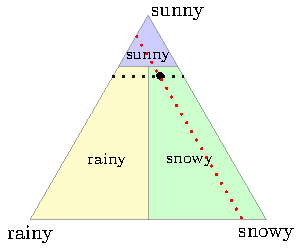
\includegraphics[width=0.5\linewidth]{tikz/t-example.pdf}
	\caption{A meteorology example with a bias towards citizen safety.}
	\label{fig:t-example}
\end{figure}


\end{document}
%%% Local Variables:
%%% mode: latex
%%% TeX-master: t
%%% End:
